\chapter{$P_N$-Method}
%
\label{sec:pnmethod}

The $P_N$-method is a deterministic method for computing light transport in a participating media. It is based on the spherical harmonics discretization of the radiative transfer equation and its related quantities in angular domain. The method has its origins in astrophysics and is also popular in nuclear sciences and medical science. It came up in the field of computer graphics only in so far that Kajia~\cite{Kajiya84} brushed over the theory, but did not give any details on implementation or how to solve it. In fact, as Max~\cite{Max95} pointed out, it is not clear if Kajiya succeeded at all at applying the method, as all of the results in his paper were produced with a simpler method\footnote{\cite{Max95} p.4: \emph{``[...] Kajiya attempted to solve these equations for the case of isotropic scattering, but it is unclear whether he succeeded, since all the pictures in \cite{Kajiya84} were produced by the simpler 'slab' method.[...]"}}. This doubt is further strengthened by results in this thesis, which show that a straight forward finite difference discretization of the $P_N$-equations produces unuseable results, due to oscillation artifacts in the solution. 
\TD{reference for pn method in astrophysics, neutron transport, medical sciences etc.}

In this chapter, we will give a thorough derivation of the $P_N$-theory. The first section introduces the spherical harmonics expansion and important properties. Then the complex-valued $P_N$-equations are derived in section~\ref{sec:pn_cvalued}. The fact, that the radiance field is positive in every direction can be used to cut the number of unknowns in half. This is done by using the real-valued $P_N$-equations. In section~\ref{sec:pn_rvalued}, a very compact form of the real-valued $P_N$-equations is derived, which has not been given anywhere else in the literature before. After a short note on two-dimensional problems in section~\ref{sec:pn_2d}, The chapter continues by introducing a new method for solving the $P_N$-equations (section~\ref{sec:pn_solver}) and closes by discussing its integration into a rendering framework and giving results (section~\ref{sec:pn_results}).

% ============================================================
\section{Spherical Harmonics}
\label{sec:sh}

Spherical harmonics are the Fourier series for the sphere, and are an important tool for solving numerical problems involving the spherical domain. They are often derived as eigensolutions to the surface Laplacian, which is the analog to developing the Fourier series as eigensolutions of the operator $(d/dx)^2$ on a finite line with the boundary conditions that $y$ and $dy/dx$ match at the two ends (see Riley et al.~\cite{Riley2006}). The result of this derivation are complex-valued functions $\SHBC$, which are defined as:
\begin{align}
\label{eq:sh_definition}
\SHBC^{l,m}(\theta, \phi)=
\begin{cases}
C^{l,m}e^{im\phi}P^{l,m}\left(\operatorname{cos}\theta\right), & \text{for $m\ge0$}\\
\left(-1\right)^m\overline{\SHBC^{l\left|m\right|}}(\theta, \phi), & \text{for $m<0$}
\end{cases}
\quad ,
\end{align}
where $P^{l,m}$ are the associated Legendre polynomials. While those can be defined in many different ways, the most numerically robust way to evaluate them is by using the following set of recurrence relations (Press et al.~\cite{Press07}):
\begin{align}
P^{0,0}\left(\operatorname{cos}\theta\right) &=
1
\  ,
\nonumber
\\
P^{m,m}\left(\operatorname{cos}\theta\right) &=
\left(2m-1\right)!!\left(1-\operatorname{cos}^2\theta\right)^\frac{m}{2}
\  ,
\nonumber
\\
P^{m+1,m}\left(\operatorname{cos}\theta\right) &=
\operatorname{cos}\theta\left(2m+1\right)P^{m,m}\left(\operatorname{cos}\theta\right)
\ 
\nonumber
\\
P^{l,m}\left(\operatorname{cos}\theta\right) &=
\frac{\operatorname{cos}\theta\left(2l-1\right)}{l-m}
P^{l-1,m}\left(\operatorname{cos}\theta\right)
-
\frac{l+m-1}{l-m}
P^{l-2,m}\left(\operatorname{cos}\theta\right)
\  .
\label{eq:sh_Plm}
\end{align}
The factor $C^{l,m}$ in equation~\ref{eq:sh_definition} is defined as
\begin{align}
\label{eq:sh_definition_C}
C^{l,m}=(-1)^m\sqrt{\frac{2l+1}{4\pi}\frac{(l-m)!}{(l+m)!}}
\end{align}
Since spherical harmonics are used in many different fields, their definition can vary and one has to be careful, when comparing them across literature. This concerns the $(-1)^m$ factor in particular, which is called the Condon-Shortley phase. Sometimes, this factor is part of the definition of the associated Legendre polynomial $P^{l,m}$ and therefore does not appear in $C^{l,m}$. More importantly, the definition of $C^{l,m}$ depends on how the spherical harmonics are expected to be normalized.
\newline
\begin{figure}[h]
\centering
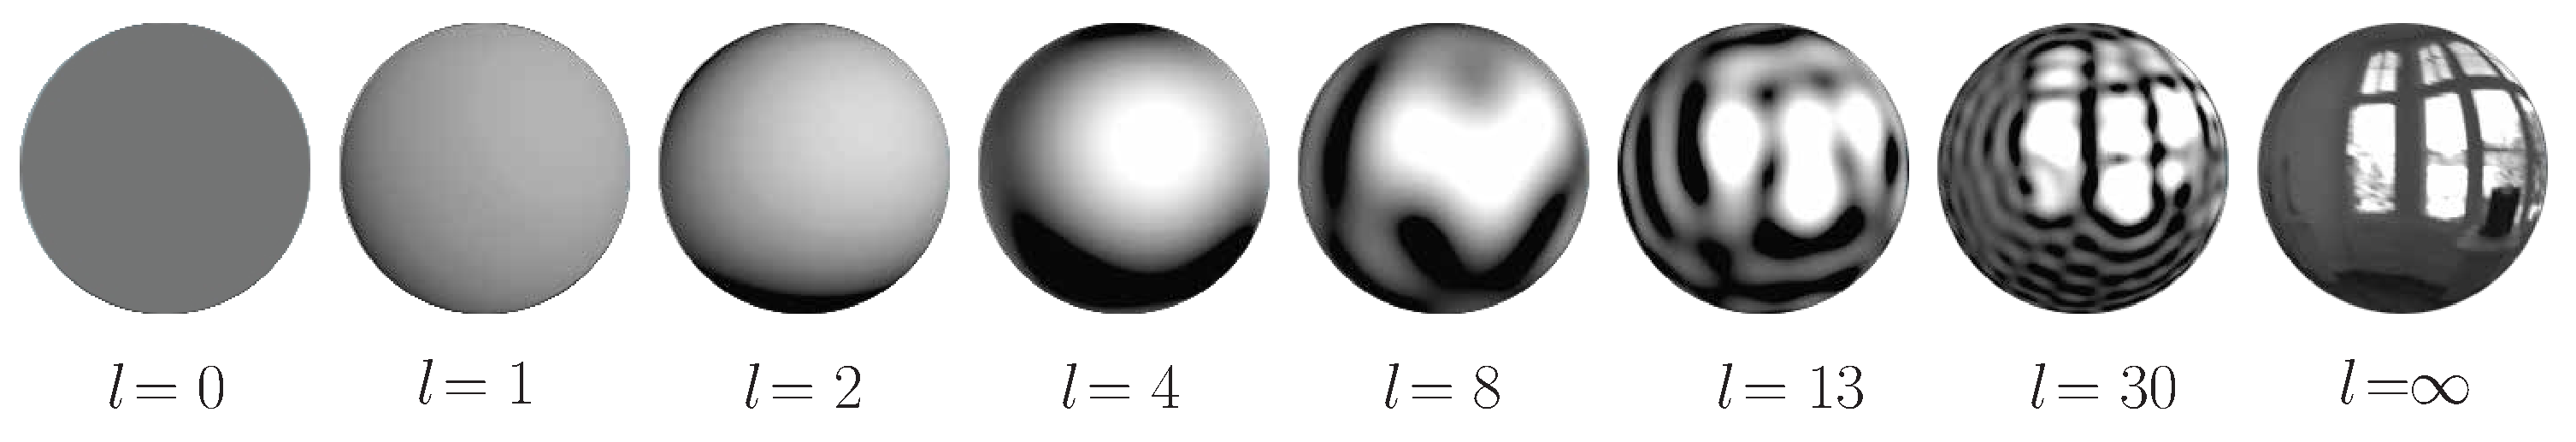
\includegraphics[width=\columnwidth]{04_pn_method/figures/fig_sph_frequencies.pdf}
\caption{Approximating a spherical function using spherical harmonics with increasing truncation order (from left to right). Like with the Fourier-transform, higher truncation order allows capturing higher frequencies.}
\label{fig:sh_vis}
\end{figure}


%\begin{figure}[h]
%\centering
%\begin{subfigure}{0.31\columnwidth}
%%\includegraphics[width=\columnwidth]{images/checkerboard2d_p1_neumann_staggered_starmap.png}
%%spherical harmonics basis function hierarchy in 2d
%\missingfigure{see comment}
%\caption{TODO}
%\label{fig:sh_vis_1}
%\end{subfigure}
%\hspace{0.01\columnwidth}
%\begin{subfigure}{0.31\columnwidth}
%%\includegraphics[width=\columnwidth]{images/checkerboard2d_p1_neumann_staggered.png}
%%some environment map and truncated reconstruction in 2d
%\missingfigure{see comment}
%\caption{TODO}
%\label{fig:sh_vis_2}
%\end{subfigure}
%\hspace{0.01\columnwidth}
%\begin{subfigure}{0.31\columnwidth}
%%\includegraphics[width=\columnwidth]{images/checkerboard2d_p1_neumann_staggered.png}
%%the hierarchy for the reconstruction with weights
%\missingfigure{see comment}
%\caption{TODO}
%\label{fig:sh_vis_3}
%\end{subfigure}%
%\caption{TODO}
%\label{fig:sh_vis}
%\end{figure}

\subsubsection*{Normalization and Orthogonality}

The coefficient $C^{l,m}$ has been defined as such that the spherical harmonics function $\SHBC$ scales to the unit norm
\begin{align}
\label{eq:sh_normalization}
\norm{\SHBC^{l,m}} = \sqrt{\left<\SHBC^{l,m}, \SHBC^{l,m}\right>} = 1
\ .
\end{align}
Other spherical harmonics definitions use a different constant (e.g. $4\pi$) and therefore arrive at different $C^{l,m}$. Since the spherical harmonics functions $\SHBC$ are complex-valued functions on the unit sphere, they are elements of the Hilbert space, for which the inner product is defined as:
\begin{align}
\label{eq:sh_inner_product}
\left<f,g\right> = \int_\Omega f\left(\vec{\omega}\right)\overline{g}\left(\vec{\omega}\right)\ud\vec{\omega}
\end{align}
with $\overline{g}$ being defined as the complex conjugate of $g$ (Folland~\cite{Folland92}).

The spherical harmonics functions form a orthogonal family and thus result in:
\begin{align}
\left<\SHBC^{l_1, m_1},\SHBC^{l_2, m_2}\right>
=
0
\ ,\quad\text{ for } l_1 \ne l_2 \text{ and } m_1 \ne m_2
\end{align}
The properties of normalization (equation~\ref{eq:sh_normalization}) and orthogonality (equation~\ref{eq:sh_orthogonality}) give
\begin{align}
\label{eq:sh_orthogonality}
\left<\SHBC^{l_1, m_1},\SHBC^{l_2, m_2}\right>=
\int_{\Omega} \SHBC^{l_1m_1}\left(\vec{\omega}\right) \overline{\SHBC^{l_2m_2}}\left(\vec{\omega}\right) \mathbf{d}\vec{\omega} = \delta_{l_1m_1}\delta_{l_2m_2}
\ .
\end{align}

\subsubsection*{Projection and Reconstruction}

Because the spherical harmonics are orthonormal, a spherical functional $f\left(\vec{\omega}\right)$ can be projected into scalar spherical harmonics basis function coefficients $f^{l,m}$, using the inner product from equation~\ref{eq:sh_inner_product}. For notational convenience the projection operator $\mathcal{P}$ shall be defined, which takes a spherical functional and returns its spherical harmonics projection for a given pair of spherical harmonics coefficients $l,m$:
\begin{align}
\label{eq:sh_projection}
\mathcal{P}^{l, m}(f) =  \left<f,\SHBC^{l, m}\right> = 
\int_\Omega f\left(\vec{\omega}\right)\overline{\SHBC^{l,m}}\left(\vec{\omega}\right)\ud\vec{\omega}
\ .
\end{align}
Note, the use of the complex conjugate $\overline{\SHBC}$ for computing the coefficients $f^{l,m}$. This comes from the definition of the inner product (equation~\ref{eq:sh_inner_product}), which is a result of Hilbert space theory. 

Given the coefficients $f^{l, m} = \mathcal{P}^{l, m}(f)$, the function $f$ can be fully reconstructed by summing up the weighted contributions from the spherical harmonics basis functions
\begin{align}
\label{eq:sh_reconstruction}
f\left(\vec{\omega}\right) = 
\sum_{l=0}^{N}
{
\sum_{m=-l}^{l}
{
f^{l,m}\left(\vec{x}\right)\SHBC^{l,m}\left(\vec{\omega}\right)
}
}
\ .
\end{align}
The function can be fully reconstructed if $N=\infty$. However, as with the Fourier-expansion, it is useful to truncate the expansion at a specific $N$ (giving $P_N$-method its name). This limits the number of coefficients at the expense of introducing an approximation error by cutting off higher frequencies. The number of sperical harmonics coefficients for truncation order $N$ is $(N+1)\times(N+1)$.

\subsubsection*{Frequency-invariant Rotation and Rotational Symmetry}

Applying a rotation to the argument of a spherical harmonics basis function of band $l$ can be expressed as a linear combination of spherical harmonics basis functions of the same order:
\begin{align}
\label{eq:sh_rotation}
\SHBC^{l,m}\left(R\vec{\omega}\right)=\sum_{j=-l}^{l}r^{l,j}\SHBC^{l,j}\left(\vec{\omega}\right)
\ .
\end{align}
This is derived from the fact that the spherical harmonics basis functions of order $l$ form an irreducible basis for the group of 3D-rotations (see Corollary $17.17$ in \cite{Hall13}). Equation~\ref{eq:sh_rotation} implies that a rotation of a function represented in spherical harmonics, does not introduce or loose any frequencies from or to other spherical harmonic bands and therefore is not subject to aliasing.

The spherical harmonics projection of a rotationally symmetric function $f$ simplifies to Zonal Spherical Harmonics, which are characterized by the fact that only coefficients with $f^{l,0}$ are needed for reconstruction. This property is needed for the derivation of the $P_N$-equations. In particular, the phase function depends only on the angle between incident direction $\vec{\omega}_i$ and outgoing direction $\vec{\omega}_o$, which means that the phase function will be rotationally symmetric around the outgoing direction, if it is fixed. 

A rotation $R(\alpha)$ of angle $\alpha$ around the pole axis is expressed in spherical harmonics as:
\begin{align*}
\rho_{R(\alpha)}(\SHBC^{l,m}) = e^{-i m\alpha}\SHBC^{l,m}
\ .
\end{align*}
If a function $f$ is rotationally symmetric around the pole axis, then following applies:
\begin{align*}
\rho_{R(\alpha)}(f) = f
\end{align*}
and in spherical harmonics this would be:
\begin{align*}
\sum_{l,m}
{
e^{-i m\alpha}
f^{l,m}
\SHBC^{l,m} }\left(\vec{\omega}\right)
=
\sum_{l,m}
{
\phase^{l,m}
\SHBC^{l,m}\left(\vec{\omega}\right)
}
\end{align*}
By equating coefficients this yields:
\begin{align*}
f^{l,m} = f^{l,m}e^{-i m\alpha}
\end{align*}
Since $e^{-i m\alpha}=1$ for all $\alpha$ only when $m=0$, the conclusion is that $f^{l,m} = 0$ for all $m\ne0$. For a function, which is rotationally symmetric around the pole axis, only the $m=0$ coefficients will be valid.

As mentioned earlier, this will be useful during the derivation of the $P_N$-equation and its scattering term in particular. If the outgoing direction $\vec{\omega}_o$ of the phase function at the north pole ($\vec{\omega}_o=\vec{e}_3$) is fixed, then the reconstruction requires exclusively the spherical harmonics coefficients with $m=0$:
\begin{align}
\label{eq:sh_exp_phase}
\phase(\vec{\omega}_i) =
\sum_l
{
\phase^{l0}
\SHBC^{l0}(\vec{\omega}_i)
}
\end{align}

\subsubsection*{Recursive Relation}

Another property, which will be important for the derivation of the $P_N$-equations and its derivative term in particular is the following recursive relation
\begin{equation}
\label{eq:recursive_relation}
\resizebox{1.0\hsize}{!}{$\vec{\omega}\overline{\SHBC^{l,m}} = \frac{1}{2}
\begin{pmatrix}
\ c^{l-1, m-1}\overline{\SHBC^{l-1,m-1}} - d^{l+1, m-1}\overline{\SHBC^{l+1,m-1}} - e^{l-1, m+1}\overline{\SHBC^{l-1,m+1}} + f^{l+1, m+1}\overline{\SHBC^{l+1,m+1}}\\
i\left(-c^{l-1, m-1}\overline{\SHBC^{l-1,m-1}} + d^{l+1, m-1}\overline{\SHBC^{l+1,m-1}} - e^{l-1, m+1}\overline{\SHBC^{l-1,m+1}} + f^{l+1, m+1}\overline{\SHBC^{l+1,m+1}}\right) \\
2\left(a^{l-1, m}\overline{\SHBC^{l-1,m}}+b^{l+1, m}\overline{\SHBC^{l+1,m}}\right)
\end{pmatrix}$}
\ ,
\end{equation}
where
\begin{equation*}
\resizebox{1.0\hsize}{!}{$
a^{l,m}= \sqrt{\frac{\left(l-m+1\right)\left(l+m+1\right)}{\left(2l+1\right)\left(2l-1\right)}} \qquad
b^{l,m}= \sqrt{\frac{\left(l-m\right)\left(l+m\right)}{\left(2l+1\right)\left(2l-1\right)}} \qquad
c^{l,m}= \sqrt{\frac{\left(l+m+1\right)\left(l+m+2\right)}{\left(2l+3\right)\left(2l+1\right)}}
$}
\end{equation*}
\begin{equation*}
\resizebox{1.0\hsize}{!}{$
d^{l,m}= \sqrt{\frac{\left(l-m\right)\left(l-m-1\right)}{\left(2l+1\right)\left(2l-1\right)}} \qquad
e^{l,m}= \sqrt{\frac{\left(l-m+1\right)\left(l-m+2\right)}{\left(2l+3\right)\left(2l+1\right)}} \qquad
f^{l,m}= \sqrt{\frac{\left(l+m\right)\left(l+m-1\right)}{\left(2l+1\right)\left(2l-1\right)}}
$}
\end{equation*}
This relation implies that a direction vector $\vec{\omega}$ scaled by a complex SH basis function $\SHBC$ of order $lm$ can be expressed as a vector of complex values basis functions of higher and lower order. Such recursion relations seem to be hard to find in the standard literature and are preserved through citations in relevant articles\footnote{according to email exchange with experts from nuclear sciences}, such as Seibold et al.~\cite{Seibold14} or Brunner et al.~\cite{Brunner05}. The signs for the $x$- and $y$- component depend on the handedness of the coordinate system, in which the spherical harmonics basis functions are defined.
\section{Complex-valued $P_N$-equations}
\label{sec:pn_cvalued}

Equipped with key properties of the spherical harmonics expansion, the complex-valued $P_N$-equations are derived in this section. The derivation follows two basic steps, which are executed separately on each term of the radiative transfer equation. The first step is to substitute each angular dependent radiative transfer quantity, such as the radiance field $L$, by its (truncated) spherical harmonics projection (equation~\ref{eq:sh_projection}). The second step is to apply the spherical harmonics projection to each term of the radiative transfer equation. This results in terms, which will depend on the spherical harmonics indices $l,m$ and therefore form a system of equations. The size of this system is driven by the truncation order $N$. The higher the value $N$, the higher frequencies in angular domain are taken into account for an approximation of the radiative transport.
% --------------------------------------------------------------
\subsubsection*{Transport Term}
The transport term of the RTE is given as
\begin{align*}
(\omega\cdot\nabla)L(\vec{x}, \omega)
\end{align*}
Replacing $L$ with its spherical harmonics expansion results in:
\begin{align*}
\left(\omega\cdot\nabla\right)
\left(
\sum_{l,m}
{
L^{l,m}\left(\vec{x}\right )
\SHBC^{l,m}\left(\omega\right)
}
\right)
\end{align*}
Next, the whole term is projected into spherical harmonics, which means a multiplication with $\overline{\SHBC^{l'm'}}$ and integration over solid angle:
\begin{align*}
\int_\Omega
{
\overline{Y^{l'm'}}(\omega\cdot\nabla)
\sum_{l,m}
{
L^{l,m}\left(\vec{x}\right)
\SHBC^{l,m}\left(\omega\right)
}
}
\ud\omega
\end{align*}
The spatial derivative can be extracted to get:
\begin{align*}
\nabla\cdot\int_\Omega
{
\omega\overline{\SHBC^{l'm'}}
\sum_{l,m}
{
L^{l,m}\left(\vec{x}\right)
\SHBC^{l,m}\left(\omega\right)
}
\ud\omega
}
\end{align*}
When applying the recursion relation (equation~\ref{eq:recursive_relation}) the following will be shown:
\begin{equation*}
\resizebox{1.0\hsize}{!}{$
\begin{pmatrix}
\frac{1}{2}\partial_x\\
\frac{i}{2}\partial_y\\
\partial_z
\end{pmatrix}
\cdot
\int_\Omega
\begin{pmatrix}
\ c^{l'-1, m'-1}\overline{\SHBC^{l'-1,m'-1}} - d^{l'+1, m'-1}\overline{\SHBC^{l'+1,m'-1}} - e^{l'-1, m'+1}\overline{\SHBC^{l'-1,m'+1}} + f^{l'+1, m'+1}\overline{\SHBC^{l'+1,m'+1}}\\
-c^{l'-1, m'-1}\overline{\SHBC^{l'-1,m'-1}} + d^{l'+1, m'-1}\overline{\SHBC^{l'+1,m'-1}} - e^{l'-1, m'+1}\overline{\SHBC^{l'-1,m'+1}} + f^{l'+1, m'+1}\overline{\SHBC^{l'+1,m'+1}} \\
a^{l'-1, m'}\overline{\SHBC^{l'-1,m'}}+b^{l'+1, m'}\overline{\SHBC^{l'+1,m'}}
\end{pmatrix}
\sum_{l,m}{
L^{l,m}\left(\vec{x}\right )\SHBC^{l,m}\left(\omega\right)
}
\ud\omega
$}
\end{equation*}
Integrating the vector term over solid angle, can be expressed as seperate solid angle integrals over each component. These integrals over a sum of terms are split into seperate integrals:
\begin{align*}
\begin{pmatrix}
\frac{1}{2}\partial_x\\
\frac{i}{2}\partial_y\\
\partial_z
\end{pmatrix}
\cdot
\begin{pmatrix}
\ c^{l'-1, m'-1}\sum_{l,m}{L^{l,m}\left(\vec{x}\right )\int_\Omega{\overline{\SHBC^{l'-1,m'-1}}\left(\omega\right)\SHBC^{l,m}\left(\omega\right)\ud\omega}} \quad - \quad ...\\
-c^{l'-1, m'-1}\sum_{l,m}{L^{l,m}\left(\vec{x}\right )\int_\Omega{\overline{\SHBC^{l'-1,m'-1}}\left(\omega\right)\SHBC^{l,m}\left(\omega\right)\ud\omega}} \quad + \quad ... \\
a^{l'-1, m'}\sum_{l,m}{L^{l,m}\left(\vec{x}\right )\int_\Omega{\overline{\SHBC^{l'-1,m'}}\left(\omega\right)\SHBC^{l,m}\left(\omega\right)\ud\omega}} \quad + \quad ...
\end{pmatrix}
\end{align*}
Applying the orthogonality property to the solid angle integrals will select specific $l,m$ in each term:
\begin{equation*}
\resizebox{1.0\hsize}{!}{$
\begin{pmatrix}
\frac{1}{2}\partial_x\\
\frac{i}{2}\partial_y\\
\partial_z
\end{pmatrix}
\cdot
\begin{pmatrix}
\ c^{l-1, m-1}L^{l-1,m-1} - d^{l+1, m-1}L^{l+1,m-1} - e^{l-1, m+1}L^{l-1,m+1} + f^{l+1, m+1}L^{l+1,m+1}\\
-c^{l-1, m-1}L^{l-1,m-1} + d^{l+1, m-1}L^{l+1,m-1} - e^{l-1, m+1}L^{l-1,m+1} + f^{l+1, m+1}L^{l+1,m+1} \\
a^{l-1, m}L^{l-1,m}+b^{l+1, m}L^{l+1,m}
\end{pmatrix}
$}
\end{equation*}
Which gives the final moment equation for the transport term:
\begin{align}
&
\frac{1}{2}c^{l-1, m-1}\partial_x L^{l-1,m-1}
-\frac{1}{2}d^{l+1, m-1}\partial_x L^{l+1,m-1}
-\frac{1}{2}e^{l-1, m+1}\partial_x L^{l-1,m+1}
\nonumber
\\
&
+\frac{1}{2}f^{l+1, m+1}\partial_x L^{l+1,m+1}
-\frac{i}{2}c^{l-1, m-1}\partial_y L^{l-1,m-1}
+\frac{i}{2}d^{l+1, m-1}\partial_y L^{l+1,m-1}
\nonumber
\\
&
-\frac{i}{2}e^{l-1, m+1}\partial_y L^{l-1,m+1}
+\frac{i}{2}f^{l+1, m+1}\partial_y L^{l+1,m+1}
+
a^{l-1, m}\partial_z L^{l-1,m}+b^{l+1, m}\partial_z L^{l+1,m}
\label{eq:sh_complex_transport}
\end{align}

% --------------------------------------------------------------
\subsubsection*{Scattering Term}

The scattering term in the RTE is given as:
\begin{align*}
\sigma_s(\vec{x})\int_{\Omega}\phase(\vec{x}, \omega'\cdot\omega)L(\vec{x}, \omega')\ud\omega'
\end{align*}
The phase function, used in isotropic scattering medium, only depends on the angle between incident and outgoing direction, and therefore is rotationally symmetric around the pole defining axis. This property allows to define a rotation $R(\omega)$, which rotates the phase function, such that the pole axis aligns with the outgoing direction vector $\omega$. This rotation is expressed as:
\begin{align*}
\rho_{R(\omega)}(\phase)
\ ,
\end{align*}
which can be implemented by applying the inverse rotation $R(\omega)^{-1}$ to the arguments of $\phase$. With this rotated phase function, the integral of the scattering operator can be expressed as a convolution:
\begin{align}
\int_{\Omega'}\phase(\vec{x}, \omega'\cdot\omega)L(\vec{x}, \omega')\ud\omega'
&=
\int_{\Omega'}{\rho_{R(\omega)}(\phase)(\operatorname{cos}\theta')L(\vec{x}, \omega')\ud\omega'}
\nonumber\\
&= \langle L,  \rho_{R(\omega)}(\phase)\rangle
\label{eq:complex_scatt_conv}
\end{align}
As the inner product integral of the convolution is evaluated, the phase function rotates along with the argument $\omega$.

Now, the spherical harmonics expansions of $L$ and $\phase$ (equation~\ref{eq:sh_exp_phase}) in the definition for the inner product of the convolution (equation~\ref{eq:complex_scatt_conv}) is used:
\begin{align*}
\langle L,  \rho_{R(\omega)}(\phase)\rangle = \left < \sum_{l,m}{L^{l,m}(\vec{x}) \SHBC^{l,m}}, \rho_{R(\omega)}\left ( \sum_{l}{\phase^{l0}\SHBC^{l0}} \right )\right>
\end{align*}
Due to linearity of the inner product operator, the non-angular dependent parts of the expansions can be pulled out:
\begin{align*}
\langle L,  \rho_{R(\omega)}(\phase)\rangle
&=
\sum_{l,m}
{
L^{l,m}(\vec{x})
\left<
\SHBC^{l,m},
\rho_{R(\omega)}
\left(\sum_l{\phase^{l0} \SHBC^{l0}}\right)
\right>
}
\end{align*}
and further:
\begin{align*}
\langle L,  \rho_{R(\omega)}(\phase)\rangle
&=
\sum_{l'}
{
\sum_{l,m}
{
\phase^{l'0}L^{l,m}(\vec{x})
\left<\SHBC^{l,m}, \rho_{R(\omega)}\left( \SHBC^{l'0} \right)\right>
}
}
\end{align*}
The rotation $\rho_{R(\omega)}$ of a function with frequency $l$ results in a function of frequency $l$ (equation~\ref{eq:sh_rotation}). In addition the spherical harmonics basis functions $\SHBC^{l,m}$ are orthogonal. Therefore following applies:
\begin{align*}
\left<
\SHBC^{l,m}, \rho_{R(\omega)}\left(\SHBC^{l'm'}\right)
\right> = 0       \qquad    \text{for all}\ \ l\ne l' 
\end{align*}
which further simplifies the inner product integral to:
\begin{align*}
\langle L,  \rho_{R(\omega)}(\phase)\rangle
&=
\sum_{l,m}
{
\phase^{l0}L^{l,m}(\vec{x})
\left<
\SHBC^{l,m}, \rho_{R(\omega)}\left(\SHBC^{l0} \right )
\right>
}
\end{align*}
What remains to be resolved is the inner product. The spherical harmonics basis functions $ \SHBC^{l,m}$ are eigenfunctions of the inner product integral operator in the equation above (Dai~\cite{Dai13}):
\begin{align*}
\left<
\SHBC^{l,m}, \rho_{R(\omega)}\left ( \SHBC^{l0} \right )\right> = \lambda_l \SHBC^{l,m}
\end{align*}
with
\begin{align*}
\lambda_l=\sqrt{\frac{4\pi}{2l+1}}
\end{align*}
Replacing the inner product leads to:
\begin{align*}
\langle L,  \rho_{R(\omega)}(p)\rangle
&=
\sum_{l,m}
{
\lambda_l
\phase^{l0}L^{l,m}(\vec{x})
\SHBC^{l,m}
}
\end{align*}
This allows to express the scattering term using SH expansions of phase function $p$ and radiance field $L$:
\begin{align*}
\sigma_s(\vec{x})\int_{\Omega}\phase(\vec{x}, \omega'\cdot\omega)L(\vec{x}, \omega')\ud\omega'
&=
\sigma_s(\vec{x})\langle L,  \rho_{R(\omega)}(p)\rangle
\\
&=
\sigma_s(\vec{x})
\sum_{l,m}
{
\lambda_l
\phase^{l0}L^{l,m}(\vec{x})
\SHBC^{l,m}
}
\end{align*}
However, a spherical harmonics expansion of the term itsself has not been done yet. It is still a scalar function that depends on direction $\omega$. The scattering term is projected into spherical harmonics, by multiplying with $\overline {\SHBC^{l'm'}}$ and integrating over solid angle $\omega$. Further all factors will be pulled out, which do not depend on $\omega$ and apply the SH orthogonality property to arrive at the scattering term of the complex-valued $P_N$-equations:
\begin{align}
&
\int_{\Omega}
{
\overline{\SHBC^{l'm'}}(\omega)
\sigma_s(\vec{x})
\sum_{l,m}
{
\lambda_l
\phase^{l0}L^{l,m}(\vec{x})
\SHBC^{l,m}\left(\omega\right)
}
\ud\omega
}
\nonumber\\
=&
\lambda_l
\sigma_s(\vec{x})
\phase^{l0}L^{l,m}(\vec{x})
\sum_{l,m}
{
\int_{\Omega}
{
\overline{\SHBC^{l'm'}}(\omega)
\SHBC^{l,m}\left(\omega\right)
\ud\omega
}
}
\nonumber\\
=&
\lambda_l
\sigma_s(\vec{x})
\phase^{l0}L^{l,m}(\vec{x})
\sum_{l,m}
{
\delta_{ll'}\delta_{mm'}
}
\nonumber\\
=&
\lambda_l
\sigma_s(\vec{x})
\phase^{l0}L^{l,m}(\vec{x})
\label{eq:sh_complex_scattering}
\end{align}



% ------------------------------------------------------------
\subsubsection*{Collision and Emission Term}

The collision term of the RTE is given as:
\begin{align*}
-\sigma_t\left(\vec{x}\right)L\left(\vec{x}, \omega\right)
\end{align*}
The radiance field $L$ is replaced with its spherical harmonics expansion:
\begin{align*}
-\sigma_t\left(\vec{x}\right)
\sum_{l,m}
{
L^{l,m}\left(\vec{x}\right )\SHBC^{l,m}\left(\omega\right)
}
\end{align*}
Multiplying with $\overline{\SHBC^{l'm'}}$ and integrating over solid angle, after pulling some factors out of the integral and applying the orthogonality identity (equation~\ref{eq:sh_orthogonality}) results in:
\begin{align}
&-\sigma_t\left(\vec{x}\right)\sum_{l,m}{L^{l,m}\left(\vec{x}\right )\int_\Omega\overline{\SHBC^{l'm'}}\left(\omega\right)\SHBC^{l,m}\left(\omega\right)\ud\omega}
\nonumber
\\
&= -\sigma_t\left(\vec{x}\right)\sum_{l,m}{L^{l,m}\left(\vec{x}\right )\delta_{ll'}\delta_{mm'}}
\nonumber
\\
&= -\sigma_t\left(\vec{x}\right)L^{l,m}\left(\vec{x}\right )
\label{eq:sh_complex_collision}
\end{align}
The derivation of the SH projected term is equal to the derivation of the projected collision term. After replacing the emission field with its SH projection and multiplying the term with the conjugate complex of $\SHBC$ results after application of the orthogonality property in:
\begin{align}
Q^{l,m}\left(\vec{x}, \omega\right)
\label{eq:sh_complex_emission}
\end{align}


% --------------------------------------------------------------
\subsubsection*{Final Equation}

The results are the complex-valued $P_N$-equations, after putting all the projected terms together (equation~\ref{eq:sh_complex_transport},~\ref{eq:sh_complex_collision},~\ref{eq:sh_complex_scattering} and~\ref{eq:sh_complex_emission}):
\begin{align}
&
\frac{1}{2}c^{l-1, m-1}\partial_x L^{l-1,m-1}
-\frac{1}{2}d^{l+1, m-1}\partial_x L^{l+1,m-1}
-\frac{1}{2}e^{l-1, m+1}\partial_x L^{l-1,m+1}
\nonumber
\\
&
+\frac{1}{2}f^{l+1, m+1}\partial_x L^{l+1,m+1}
-\frac{i}{2}c^{l-1, m-1}\partial_y L^{l-1,m-1}
+\frac{i}{2}d^{l+1, m-1}\partial_y L^{l+1,m-1}
\nonumber
\\
&
-\frac{i}{2}e^{l-1, m+1}\partial_y L^{l-1,m+1}
+\frac{i}{2}f^{l+1, m+1}\partial_y L^{l+1,m+1}
+a^{l-1, m}\partial_z L^{l-1,m}
+b^{l+1, m}\partial_z L^{l+1,m}
\nonumber
\\
&
=
-\sigma_t\left(\vec{x}\right)L^{l,m}\left(\vec{x}\right )
+
\lambda_l
\sigma_s(\vec{x})
\phase^{l0}L^{l,m}(\vec{x}) + Q^{l,m}\left(\vec{x}, \omega\right)
\label{eq:sh_pne_complex}
\end{align}
\section{Real-valued $P_N$-equations}
\label{sec:pn_rvalued}

Depending on the truncation value $N$, the complex-valued $P_N$-equations will induce a certain number of spherical harmonics coefficients for every discretized position within the domain. These will be complex and therefore produce two unknowns per coefficient. Moreover, the whole pipeline from solver to rendering integration will have to deal with complex numbers. This is an unnecessary burden, as we actually only have real-valued radiance fields and volumetric quantities in rendering.

If the spherical harmonics projected function or operator is real-valued, then the resulting projection will have a redundant structure which allows cutting the number of coefficients in half. The real-valued spherical harmonics basis function (denoted $\SHBR$) can be defined by projecting these remaining coefficients onto their real and imaginary parts:
% real valued SH ------------------
\begin{align}
\label{eq:real_sh_basis}
\SHBR^{l,m}=
\left\{
\begin{array}{lr}
\frac{\iu}{\sqrt{2}}\left(\SHBC^{l,m}-\left(-1\right)^m\SHBC^{l,-m}\right), & \text{for } m < 0\\
\SHBC^{l,m}, & \text{for } m = 0\\
\frac{1}{\sqrt{2}}\left(\SHBC^{l,-m}+\left(-1\right)^m\SHBC^{l,m}\right), & \text{for } m > 0
\end{array}
\right.
\end{align}
Therfore the number of spherical harmonics coefficients remains the same, but since those are now real only, the number of unknowns is cut in half.

In this section, the real-valued $P_N$-equations are derived by using $\SHBR$ instead of $\SHBC$ for the derivation. This allows to get rid of complex numbers everywhere in the pipeline and reduces the amount of unknowns. The real-valued $P_N$-equations as such are not new. However, performing the derivation steps manually produces very large equations which are hard to work with and make it very difficult to see structures and opportunities for simplification. Therefore in the literature, the real-valued $P_N$-equations are usually specified in form of the complex-valued $P_N$-equations in matrix form with an additional transformation matrix, representing the projection to real-valued spherical harmonics from equation~\ref{eq:real_sh_basis} (see Seibold et al.~\cite{Seibold14}). An explicit form of the real-valued $P_N$-equation cannot be found in the literature. An attempt to derive such a form has been made by Frank et al.~\cite{Frank14} (appendix A), but their result still requires matrix notation with unwieldy coefficient matrices. 

In this thesis a new explicit form of the real-valued $P_N$-equations is derived, which is very concise and compact. This derivation was made possible by using the computer algebra representation framework which has been developed as part of the solver (see section~\ref{sec:pn_car}). The derivation steps for the $P_N$-equations were carried out using this representation and simplification opportunities could be discovered much more easily, leading to the compact form presented at the end of this section.

Being real-valued implies that no complex-conjugate is needed for the inner product. The projection into real-valued spherical harmonics therefore is
\begin{align}
\label{eq:sh_projection}
f^{l, m} = \left<f,\SHBR^{l, m}\right> = 
\int_\Omega f\left(\omega\right)\SHBR^{l,m}\left(\omega\right)\ud\omega
\ .
\end{align}
All properties of the complex-valued spherical harmonics basis functions, except the recursion relation in equation~\ref{eq:recursive_relation}, carry through to the real-valued basis functions. In particular, the orthognality property still holds:
\begin{align}
\label{eq:sh_orthogonality_real}
\left<\SHBR^{l_1, m_1},\SHBR^{l_2, m_2}\right>=
\int_{\Omega} \SHBR^{l_1m_1}\left(\omega\right) \SHBR^{l_2m_2}\left(\omega\right) \mathbf{d}\omega = \delta_{l_1m_1}\delta_{l_2m_2}
\ .
\end{align}

% --------------------------------------------------------------
\subsubsection*{Transport Term}

Carrying out the derivation for the transport term of the radiative transfer equation produces very different terms compared to the complex-valued counterpart. The derivation is extensive and given in appendix~\ref{app:rpn}. As the spherical harmonics basis functions are different depending on the sign of $m$ (see equation~\ref{eq:real_sh_basis}), the projected transport term is also different accordingly. After carrying out the derivation steps we arrive for $m<0$ at:
\begin{align*}
&-\frac{1}{2}c^{{l-1,m-1}}
\partial_y
L^{l-1,-m+1}
%\\
+\frac{1}{2}d^{{l+1,m-1}}
\partial_y
L^{l+1,-m+1}
%\\
-\frac{1}{2}\beta^{m}e^{{l-1,m+1}}
\partial_y
L^{l-1,-m-1}
\\&
+\frac{1}{2}\beta^{m}f^{{l+1,m+1}}
\partial_y
L^{l+1,-m-1}
%\\
+\frac{1}{2}c^{{l-1,m-1}}
\partial_x
L^{l-1,m-1}
\\&
-\frac{1}{2}\delta_{\scaleto{m\neq -1}{4pt}}e^{{l-1,m+1}}
\partial_x
L^{l-1,m+1}
%\\
+\frac{1}{2}\delta_{\scaleto{m\neq -1}{4pt}}f^{{l+1,m+1}}
\partial_x
L^{l+1,m+1}
%\\
-\frac{1}{2}d^{{l+1,m-1}}
\partial_x
L^{l+1,m-1}
\\&
+a^{{l-1,m}}
\partial_z
L^{l-1,m}
%\\
+b^{{l+1,m}}
\partial_z
L^{l+1,m}
\end{align*}
with
\begin{align}
\label{eq:real_sh_basis}
\beta^{x}=
\left\{
\begin{array}{lr}
\frac{2}{\sqrt{2}}, & \text{for } \vert x\vert = 1\\
1, & \text{for } \vert x\vert \neq 1
\end{array}
\right.
\end{align}
Following the derivation through for $m>0$ gives:
\begin{align}
&
\frac{1}{2}c^{l-1,-m-1}\partial_x L^{l-1,m+1}
%\\&
-\frac{1}{2}d^{l+1,-m-1}\partial_x L^{l+1,m+1}
%\\&
-\frac{1}{2}\beta^{m}e^{l-1,m-1}\partial_x L^{l-1,m-1}
\nonumber
\\&
\frac{1}{2}\beta^{m}f^{l+1,-m+1}\partial_x L^{l+1,m-1}
%\\&
\frac{1}{2}c^{l-1,-m-1}\partial_y L^{l-1,-m-1}
%\\&
-\frac{1}{2}d^{l+1,-m-1}\partial_y L^{l+1,-m-1}
\nonumber
\\&
\delta_{\scaleto{m\neq 1}{4pt}}\frac{1}{2}e^{l-1,-m+1}\partial_y L^{l-1,-m+1}
%\\&
-\delta_{\scaleto{m\neq 1}{4pt}}\frac{1}{2}f^{l+1,-m+1}\partial_y L^{l+1,-m+1}
%\\&
a^{l-1,-m}\partial_z L^{l-1,m}
\nonumber
\\&
b^{l+1,-m}\partial_z L^{l+1,m}
\nonumber
\end{align}
Similar simplifications apply to the remaining terms of the spherical harmonics expansion of the transport term for $m=0$, resulting in the expression:
\begin{align}
\label{eq:pn_rvalued_transport_m0}
&
\frac{1}{\sqrt{2}}c^{{l-1,-1}}\partial_x L^{{l-1,1}}
-\frac{1}{\sqrt{2}}d^{{l+1,-1}}\partial_x L^{{l+1,1}}
\\&
\frac{1}{\sqrt{2}}c^{{l-1,-1}}\partial_y L^{{l-1,-1}}
-\frac{1}{\sqrt{2}}d^{{l+1,-1}}\partial_y L^{{l+1,-1}}
\\&
a^{{l-1,0}}\partial_z L^{{l-1,0}}
+b^{{l+1,0}}\partial_z L^{{l+1,0}}
\end{align}

% --------------------------------------------------------------
\subsubsection*{Collision, Scattering and Emission}

The remaining terms of the radiative transfer equation are derived in the same way, as their complex-valued counterpart. The collision term for $m < 0$, $m=0$ and $m > 0$ is
\begin{align}
\label{eq:pn_rvalued_transport_collision}
-\sigma_t L^{l,m}
\ .
\end{align}
We have for the scattering term
\begin{align}
\label{eq:pn_rvalued_transport_scattering}
\sigma_s\lambda_{l}p^{l,0}\left(\vec{x}\right)L^{l,m}
\end{align}
and finally for the emission term
\begin{align}
\label{eq:pn_rvalued_transport_emission}
Q^{l,m}
\ .
\end{align}

% --------------------------------------------------------------
\subsubsection*{Final Equation}

By putting equation~\ref{eq:pn_rvalued_transport_m0}, equation~\ref{eq:pn_rvalued_transport_collision}, equation~\ref{eq:pn_rvalued_transport_scattering} and equation~\ref{eq:pn_rvalued_transport_emission} together we get for $m=0$:
\begin{align}
&
\frac{1}{\sqrt{2}}c^{\scaleto{l-1,-1}{4pt}}\partial_x L^{\scaleto{l-1,1}{4pt}}
-\frac{1}{\sqrt{2}}d^{\scaleto{l+1,-1}{4pt}}\partial_x L^{\scaleto{l+1,1}{4pt}}
%\\&
\frac{1}{\sqrt{2}}c^{\scaleto{l-1,-1}{4pt}}\partial_y L^{\scaleto{l-1,-1}{4pt}}
\nonumber
\\&
-\frac{1}{\sqrt{2}}d^{\scaleto{l+1,-1}{4pt}}\partial_y L^{\scaleto{l+1,-1}{4pt}}
%\\&
+a^{\scaleto{l-1,0}{4pt}}\partial_z L^{\scaleto{l-1,0}{4pt}}
+b^{\scaleto{l+1,0}{4pt}}\partial_z L^{\scaleto{l+1,0}{4pt}}
\nonumber
\\&
=
-\sigma_t L^{\scaleto{l,m}{4pt}}
+\sigma_s\lambda_{\scaleto{l}{4pt}}p^{\scaleto{l,0}{4pt}}L^{\scaleto{l,m}{4pt}}
+ Q^{\scaleto{l,m}{4pt}}
%\label{eq:rpn_m_=_z}
\end{align}
We can compact the equations for $m<0$ and $m>0$ into a single expression by differentiating the signs using $\pm$. The  top sign is associated with $m<0$ and for $m>0$ we use the bottom sign. This results in the real-valued $P_N$-equation for $m<0$ and $m>0$:
\begin{align}
&
\frac{1}{2}c^{\scaleto{l-1,\pm m-1}{4pt}}\partial_x L^{\scaleto{l-1,m\mp 1}{4pt}}
%\\&
-\frac{1}{2}d^{\scaleto{l+1,\pm m-1}{4pt}}\partial_x L^{\scaleto{l+1,m\mp 1}{4pt}}
%\\&
-\frac{1}{2}\beta_x^{\scaleto{m}{4pt}}e^{\scaleto{l-1,m\pm 1}{4pt}}\partial_x L^{\scaleto{l-1,m\pm 1}{4pt}}
\nonumber
\\&
+\frac{1}{2}\beta_x^{\scaleto{m}{4pt}}f^{l+1,\pm m+1}\partial_x L^{\scaleto{l+1,m\pm 1}{4pt}}
%\\&
\mp \frac{1}{2}c^{\scaleto{l-1,\pm m-1}{4pt}}\partial_y L^{\scaleto{l-1,-m\pm 1}{4pt}}
\nonumber
\\&
\pm \frac{1}{2}d^{\scaleto{l+1,\pm m-1}{4pt}}\partial_y L^{\scaleto{l+1,-m \pm 1}{4pt}}
%\nonumber
%\\&
\mp \beta_y^{\scaleto{m}{4pt}}\frac{1}{2}e^{\scaleto{l-1,\pm m+1}{4pt}}\partial_y L^{\scaleto{l-1,-m\mp 1}{4pt}}
\nonumber
\\&
\pm \beta_y^{\scaleto{m}{4pt}}\frac{1}{2}f^{\scaleto{l+1,\pm m+1}{4pt}}\partial_y L^{\scaleto{l+1,-m\mp 1}{4pt}}
%\\&
+a^{\scaleto{l-1,\pm m}{4pt}}\partial_z L^{\scaleto{l-1,\mp m}{4pt}}
%\nonumber
%\\&
+b^{\scaleto{l+1,\pm m}{4pt}}\partial_z L^{\scaleto{l+1,\mp m}{4pt}}
\nonumber
\\&
=
-\sigma_t L^{\scaleto{l,m}{4pt}}
+\sigma_s\lambda_{\scaleto{l}{4pt}}p^{\scaleto{l,0}{4pt}}L^{\scaleto{l,m}{4pt}}
+Q^{\scaleto{l,m}{4pt}}
%\nonumber
%\label{eq:rpn_m_>_z}
\end{align}
with
\begin{align*}
%\label{eq:real_sh_basis}
\beta_x^{m}=
\left\{
\begin{array}{ll}
0, & \text{for } m = -1\\
\frac{2}{\sqrt{2}}, & \text{for } m \neq 1\\
1, & \text{otherwise }
\end{array}
\right.
,\quad
\beta_y^{m}=
\left\{
\begin{array}{ll}
\frac{2}{\sqrt{2}}, & \text{for } m = -1\\
0, & \text{for } m \neq 1\\
1, & \text{otherwise }
\end{array}
\right.
\end{align*}
and
\begin{align*}
&
a^{\scaleto{l,m}{4pt}}= \sqrt{\frac{\left(l-m+1\right)\left(l+m+1\right)}{\left(2l+1\right)\left(2l-1\right)}} \qquad
b^{\scaleto{l,m}{4pt}}= \sqrt{\frac{\left(l-m\right)\left(l+m\right)}{\left(2l+1\right)\left(2l-1\right)}}
\\&
c^{\scaleto{l,m}{4pt}}= \sqrt{\frac{\left(l+m+1\right)\left(l+m+2\right)}{\left(2l+3\right)\left(2l+1\right)}} \qquad
d^{\scaleto{l,m}{4pt}}= \sqrt{\frac{\left(l-m\right)\left(l-m-1\right)}{\left(2l+1\right)\left(2l-1\right)}}
\\&
e^{\scaleto{l,m}{4pt}}= \sqrt{\frac{\left(l-m+1\right)\left(l-m+2\right)}{\left(2l+3\right)\left(2l+1\right)}} \qquad
f^{\scaleto{l,m}{4pt}}= \sqrt{\frac{\left(l+m\right)\left(l+m-1\right)}{\left(2l+1\right)\left(2l-1\right)}}
\end{align*}
\begin{align*}
\lambda_l=\sqrt{\frac{4\pi}{2l+1}}
\end{align*}










\section{Two-dimensional problems}
\label{sec:pn_2d}

Working with three-dimensional problems is computationally demanding and makes debugging and visualization difficult. It is therefore common practice in other fields to study and validate ideas on the $P_N$-equations for two-dimensional problems. The derivation of the two-dimensional $P_N$-equation is simple and will be given in this section.

Consider a domain in the two-dimensional space $\mathbb{R}^2$, which is extruded infinitely along the $z-axis$ in both directions into $\mathbb{R}^3$. Now we further assume that input fields, such as $\sigma_t$, and boundary conditions also do not change along the $z$-axis.

Since the domain has infinite extent in $z$-direction, the radiance field $L$ will not change along the $z$-axis at any position within the domain. Further, the upper hemisphere of the spherical radiance function will be a mirrored version of the lower hemisphere, with the equator being the mirror plane. In mathematical terms this is expressed as $L$ being an even function in the polar angle $\theta$.

From the definition of the Associated Legendre Polynomials (see equation~\ref{eq:sh_Plm}) it can be concluded that they are either even or odd according to
\begin{align}
P^{l,m}\left(-\operatorname{cos}\theta\right) = 
\left(-1\right)^{l+m}
P^{l,m}\left(\operatorname{cos}\theta\right)
\ .
\end{align}
If $l+m$ is odd, then $P^{l,m}$ is odd. This means that it integrates to zero over a symmetric interval around the origin, such as the polar angle range. Since the spherical harmonics basis functions scales $P^{lm}$ only uniformly and along the azimuthal angle, it can be infered that the spherical harmonics basis functions are odd in the polar angle $\theta$ if $l+m$ is odd.

The spherical harmonics projection of the radiance field consists of multiplying the radiance field with the spherical harmonics basis function and integrating over solid angle. This is done for each spherical harmonics coefficient ($l,m$-pair) required. We established that if $l+m$ is odd, the basis function will be odd in $\theta$. Since the radiance field is even in theta, this means that their product will be odd. This implies that the integral of their product over the polar angle range will be zero.

This means that the spherical harmonics coffeficients of $L$ will be zero for all coefficients where $l+m$ is odd. We further can set all occurances of $\partial_z$ in the $P_N$-equations to zero.


\section{$P_N$-Solver with Automated Stencil Generation}
\label{sec:pn_solver}

In this section, a new method for solving the $P_N$-equations is being given. This method is based on the idea of automatically generating the linear system of equations directly from a computer algeba representation of the $P_N$-equations. This section will go through the manual steps required to build such a system from general partial differential equations, followed by the motivation for the automated approach taken in this thesis. In subsections~\ref{sec:pn_car} to~\ref{sec:pn_staggered}, the solver and the automation of the individual system-building steps are explained in detail, including the developed software framework and important numerical aspects, such as handling boundary conditions and staggered grids.

There are three reasons why the solver has been designed around the idea of automatic system building. The first reason is that the number of equations of the system depends on the user parameter $N$ (the spherical harmonics truncation order) and is therefore not known in advance during solver implementation. Secondly, the number of equations increases quadratically with truncation order $N$, which makes manual construction of the system increasingly laborious, time consuming, and error-prone.

The third reason is that there exists a variety of variations of the $P_N$-method in other fields, which deal with different aspects of $P_N$-theory, such as reduction of ringing artefacts and improvement of convergence. Such variations include Simplified-$P_N$ ($SP_N$)~\cite{Ryan10}, Filtered-$P_N$ ($FP_N$)~\cite{Radice13}, Diffusion-Correction-$P_N$ ($DP_N$)~\cite{Schaefer11} and Least-Squares-$P_N$ ($LSP_N$)~\cite{Hansen14}. Common to all these variations is that they reduce to a set of coupled partial differential equations. The idea behind the design of the solver in this thesis is to be able to generate the coefficient matrix and right hand side vector directly from the specification of such a coupled system of equations. This would allow easy implementation and cross-comparisons of these alternate theories from the literature.

The $P_N$-equations have been derived in previous sections by discretizing the continuous angular variable in the radiative transfer equation. This led to a discrete set of coupled partial differential equations, which still depend on the continuous spatial variable~$\vec{x}$. Therefore, the next step is to discretize this spatial variable on a particular domain with input fields for the various radiative quantities, such as extinction or the phase function. Finally, using this discretization, a system of linear equations can be built by assembling a coefficient matrix $A$ and a right hand side vector~$\vec{b}$.

We will now summarize the steps for building a linear system from a given partial difference equation (using the two-dimensional Laplace equation as example). The next subsections then will revisit each step and elaborate on how it has been automated as part of the solver.

\subsubsection*{Spatial Discretization}

As mentioned in section~\ref{sec:foundations_deterministic}, a discrete representation of the geometry that covers the problem domain is required in order to discretize the spatial variable. Throughout this thesis, a regular Cartesian grid is used, which will be referred to as a finite difference grid. This type of grid is simple and commonly used in graphics. In future it might be worth exploring other complex meshes, such as tetrahedral irregular grids, which are often used in the finite element analysis. 

The finite difference grid defines the locations at which radiative transfer quantities and the solution will be specified. It is parameterized by a worldspace bounding box and a resolution $res=(I$, $J,$ $K)$ or gridspacing $h=(h_x$, $h_y,$ $h_z)$ in each dimension. The local space of the grid is referred to as a voxelspace.

Using finite difference grids, the discretization consists of replacing quantities, which depend on the continuous variable~$\vec{x}$ with its discrete counterpart $x_{ijk}$, where $ijk$ is a coordinate in voxelspace. This coordinate is still continuous and $x_{i+\frac{1}{2}jk}$ is a valid coordinate. Quantities around grid point locations are found by interpolation. In this thesis a trilinear interpolation for three-dimensional grids and bilinear interpolation for two-dimensional grids will be used. Higher order interpolation would be possible and an avenue for future exploration.
\begin{figure}[h]
\centering
%\missingfigure{image of finite difference grid showing domain, and gridpoints and indices and voxelsize h, and interpolation}
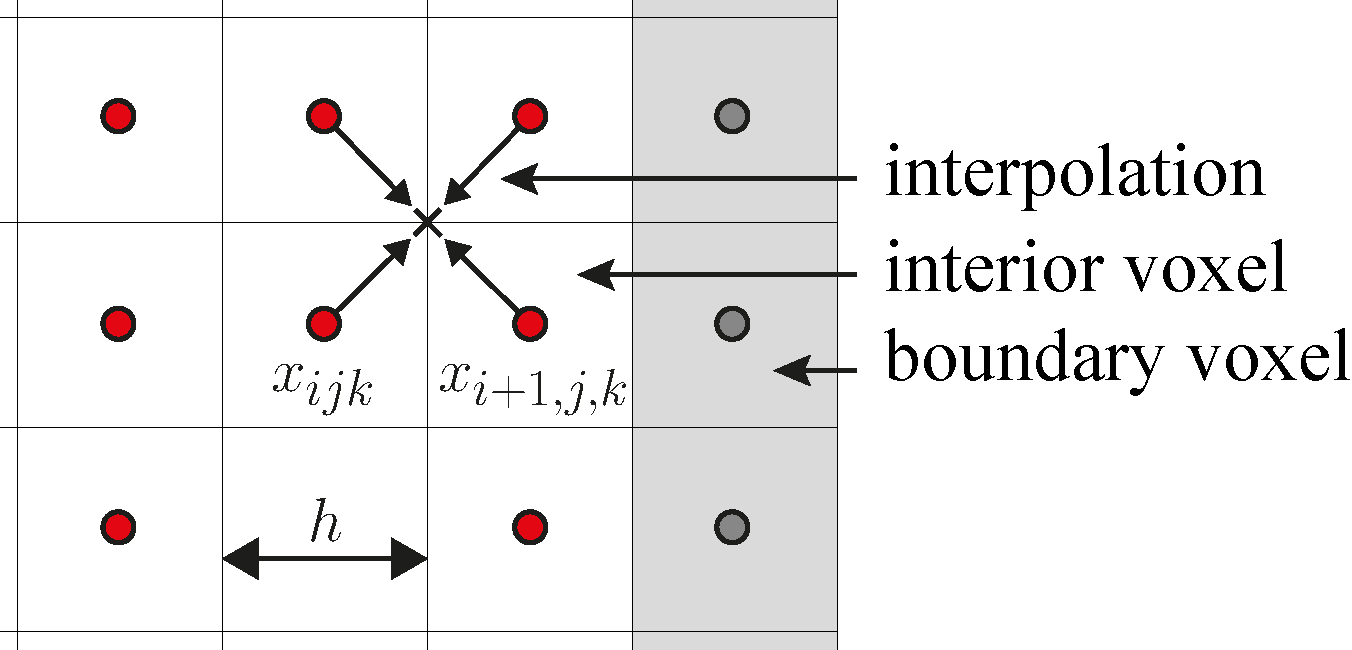
\includegraphics[width=0.6\textwidth]{04_pn_method/figures/fig_fd_grids.pdf}
\caption{Image of finite difference grid showing domain (white cells), boundary (gray cells), gridpoints (red), voxelsize $h$ and interpolation.}
\label{fig:pn_solver_finite_difference_grid}
\end{figure}

The first step during a discretization is the replacement of $\vec{x}$ by its discrete counterpart $x_{ijk}$. Using the two-dimensional Laplace equation $\nabla^2\phi(\vec{x})=q(\vec{x})$ as an example, this results in:
\begin{align*}
\nabla^2\phi\left(\vec{x}\right)=q\left(\vec{x}\right)
\xrightarrow{\vec{x} = x_{ijk}}
\partial_x^2\phi_{ij}+
\partial_y^2\phi_{ij}
=
q_{ij}
\end{align*}
For notational convenience $\phi_{ijk} = \phi\left(x_{ijk}\right)$ is defined. The spatial derivatives are approximated using central differences:
\begin{align}
\partial_x\phi_{ijk} = \frac{\phi_{i+\frac{1}{2}jk} - \phi_{i-\frac{1}{2}jk}}{h_x}
\label{eq:pn_solver_central_difference}
\end{align}
Continuing with the Laplace example, the substitutions of spatial derivatives are carried out next. Nested derivatives affect the indices accordingly:
\begin{align}
&
\xrightarrow{\text{central difference}}
\left(
\frac
{
\partial_x
\phi_{i+\frac{1}{2}j}
-
\partial_x
\phi_{i-\frac{1}{2}j}
}
{h_x}
\right)
-
\left(
\frac
{
\partial_y
\phi_{ij+\frac{1}{2}}
-
\partial_y
\phi_{ij-\frac{1}{2}}
}
{h_y}
\right)
=
q_{ij}
\nonumber
\\
&
\xrightarrow{\text{central difference}}
\frac
{
\frac{\phi_{i+1j} - \phi_{ij}}{h_x}
-
\frac{\phi_{ij} - \phi_{i-1j}}{h_x}
}
{h_x}
-
\frac
{
\frac{\phi_{ij+1} - \phi_{ij}}{h_y}
-
\frac{\phi_{ij} - \phi_{ij-1}}{h_y}
}
{h_y}
=
q_{ij}
\label{eq:laplace-central-difference}
\end{align}

\subsubsection*{Canonical Form}
After application of the discretization, equation \ref{eq:laplace-central-difference} is further brought into canonical form, which means that it is factorized according to the unknowns $\phi_{ij}$. This results in the discretized Laplace equation:
\begin{align}
\xrightarrow{\text{factorization}}
\frac{1}{h_x^2}\phi_{i+1j}
+\frac{1}{h_x^2}\phi_{i-1j}
+\frac{1}{h_y^2}\phi_{ij+1}
+\frac{1}{h_y^2}\phi_{ij-1}
-2\left(\frac{1}{h_x^2}+\frac{1}{h_y^2}\right)\phi_{ij}
=
q_{ij}
\label{eq:pn_laplace_canonical_form}
\end{align}

\subsubsection*{Stencil Code Crafting}

Consequently, the canonical form is used to derive the stencil code. This is done by interpreting the equation as a product between a row in the coefficient matrix $A$ and the vector of unknowns (the solution vector $\vec{u}$), resulting in the right hand side $q_{ij}$. The regular structure of the discretization reveals a pattern, which is the same for every row and is called a stencil code.

\begin{figure}[h]
\centering
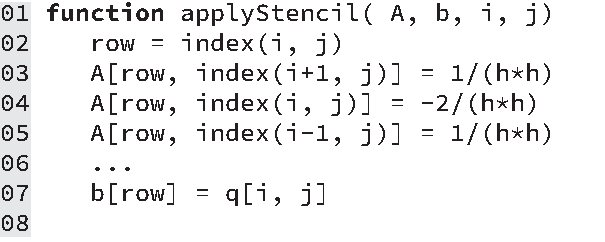
\includegraphics[width=0.6\textwidth]{04_pn_method/figures/fig_code_stencil.pdf}
%\missingfigure{source code figure for simple stencil code}
\caption{Spatial discretization of partial differential equations will lead to stencil code which is executed to populate the system matrix $A$ and right hand side vector $b$.}
\label{fig:pn_solver_stencil_code}
\end{figure}

The purpose of the stencil code is to be executed repeatedly to populate the system matrix $A$ and right hand side $\vec{b}$. This requires a mapping of multi-dimensional indices $ijk$ to linear indices into rows of $\vec{u}$ (and columns of $A$). This mapping is referred to as the \emph{index} function. The components of the solution vector $\vec{u}$ are associated with unknowns at specific grid locations $ijk$. In case of the Laplace example this would be written as:
\begin{align}
u_{\operatorname{index}\left(ijk\right)} = \phi_{ijk}\quad\text{ with }\quad \operatorname{index}: \mathbb{Z}^3\mapsto\mathbb{Z}
\label{eq:pn_index_mapping}
\end{align}

Also functions for accessing discretized input fields (such as $q$ in the Laplace example) and parameters, such as the voxel size $h$, will be called by the stencil code to retrieve required values.

\subsubsection*{System Matrix Population and Solve}
The stencil code is compiled once and then executed for each row in $A$ to populate the system. Different standard methods for solving the linear system $A\vec{u}=\vec{b}$ can be applied to find the solution $\vec{u}$, the discretized radiance field. This solution can then be used in a rendering application.
\begin{figure}[h]
\centering
%\missingfigure{image overview of the numerical pipeline}
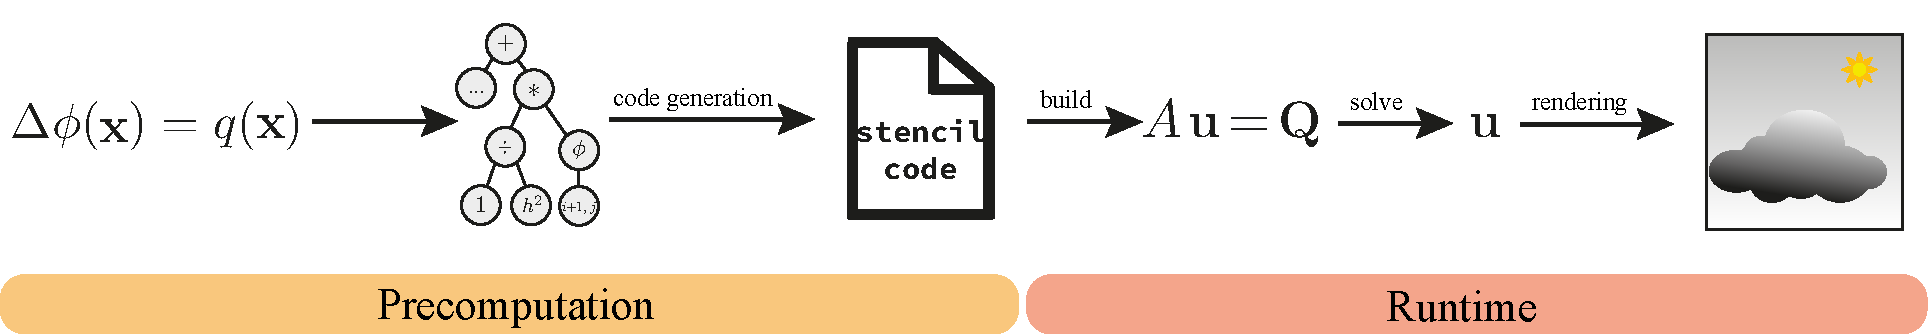
\includegraphics[width=1.0\textwidth]{04_pn_method/figures/fig_pipeline.pdf}
\caption{Overview of the method for solving the $P_N$-equations which is introduced in this chapter. The core idea is to automate the stencil code generation using a computer algebra representation of the equations.}
\label{fig:pn_solver_stencil_overview}
\end{figure}

In the following subsections, the new solver will be introduced as as a general framwork for automization of the steps for system building. The first subsection discusses how a computer algebra representation is used to represent the equation to be solved. Subsection~\ref{sec:pn_stencil_gen} shows how the spatial discretization and stencil code generation are modeled as operations on that representation. Subsection~\ref{sec:pn_bc} explains the aspects of the system that are related to boundary conditions, followed by subsection~\ref{sec:pn_framework} which discusses the surrounding framework and how the generated stencil is used within that framework. Subsection~\ref{sec:pn_staggered} elaborates on the extension of the solver to staggered grids, which is necessary for the solver to produce useful results. Finally, subsection~\ref{sec:pn_system_matrix} is dedicated to properties of the coefficient matrix $A$ and methods for solving the linear system.

\subsection{Computer Algebra Representation}
\label{sec:pn_car}

At the core of the solver is a computer algebra representation of the equations, which the system is trying to solve on a given domain. This representation is a mathematical expression tree (Preiss~\cite{Preiss00}). Each node within that tree can have any number of children and represents a constant, mathematical symbol or a mathematical operation, such as integration, derivation, power, addition or multiplication. Representations of complex equations are constructed by nesting nodes into a larger tree, where child nodes are considered as arguments of the operation, represented by the parent node.

A number of computer algebra systems exist, such as SymPy~\cite{Meurer17}, which allow to generate and manipulate computer algebra representations. However, for this thesis a small lightweight computer algebra representation containing the required subset has been developed. Figure~\ref{fig:pn_math_expression_tree_generation} demonstrates how this system is used to build the expression trees for the examples above.
\begin{figure}[h]
\centering
%\missingfigure{code listing showing how the expression tree is build}
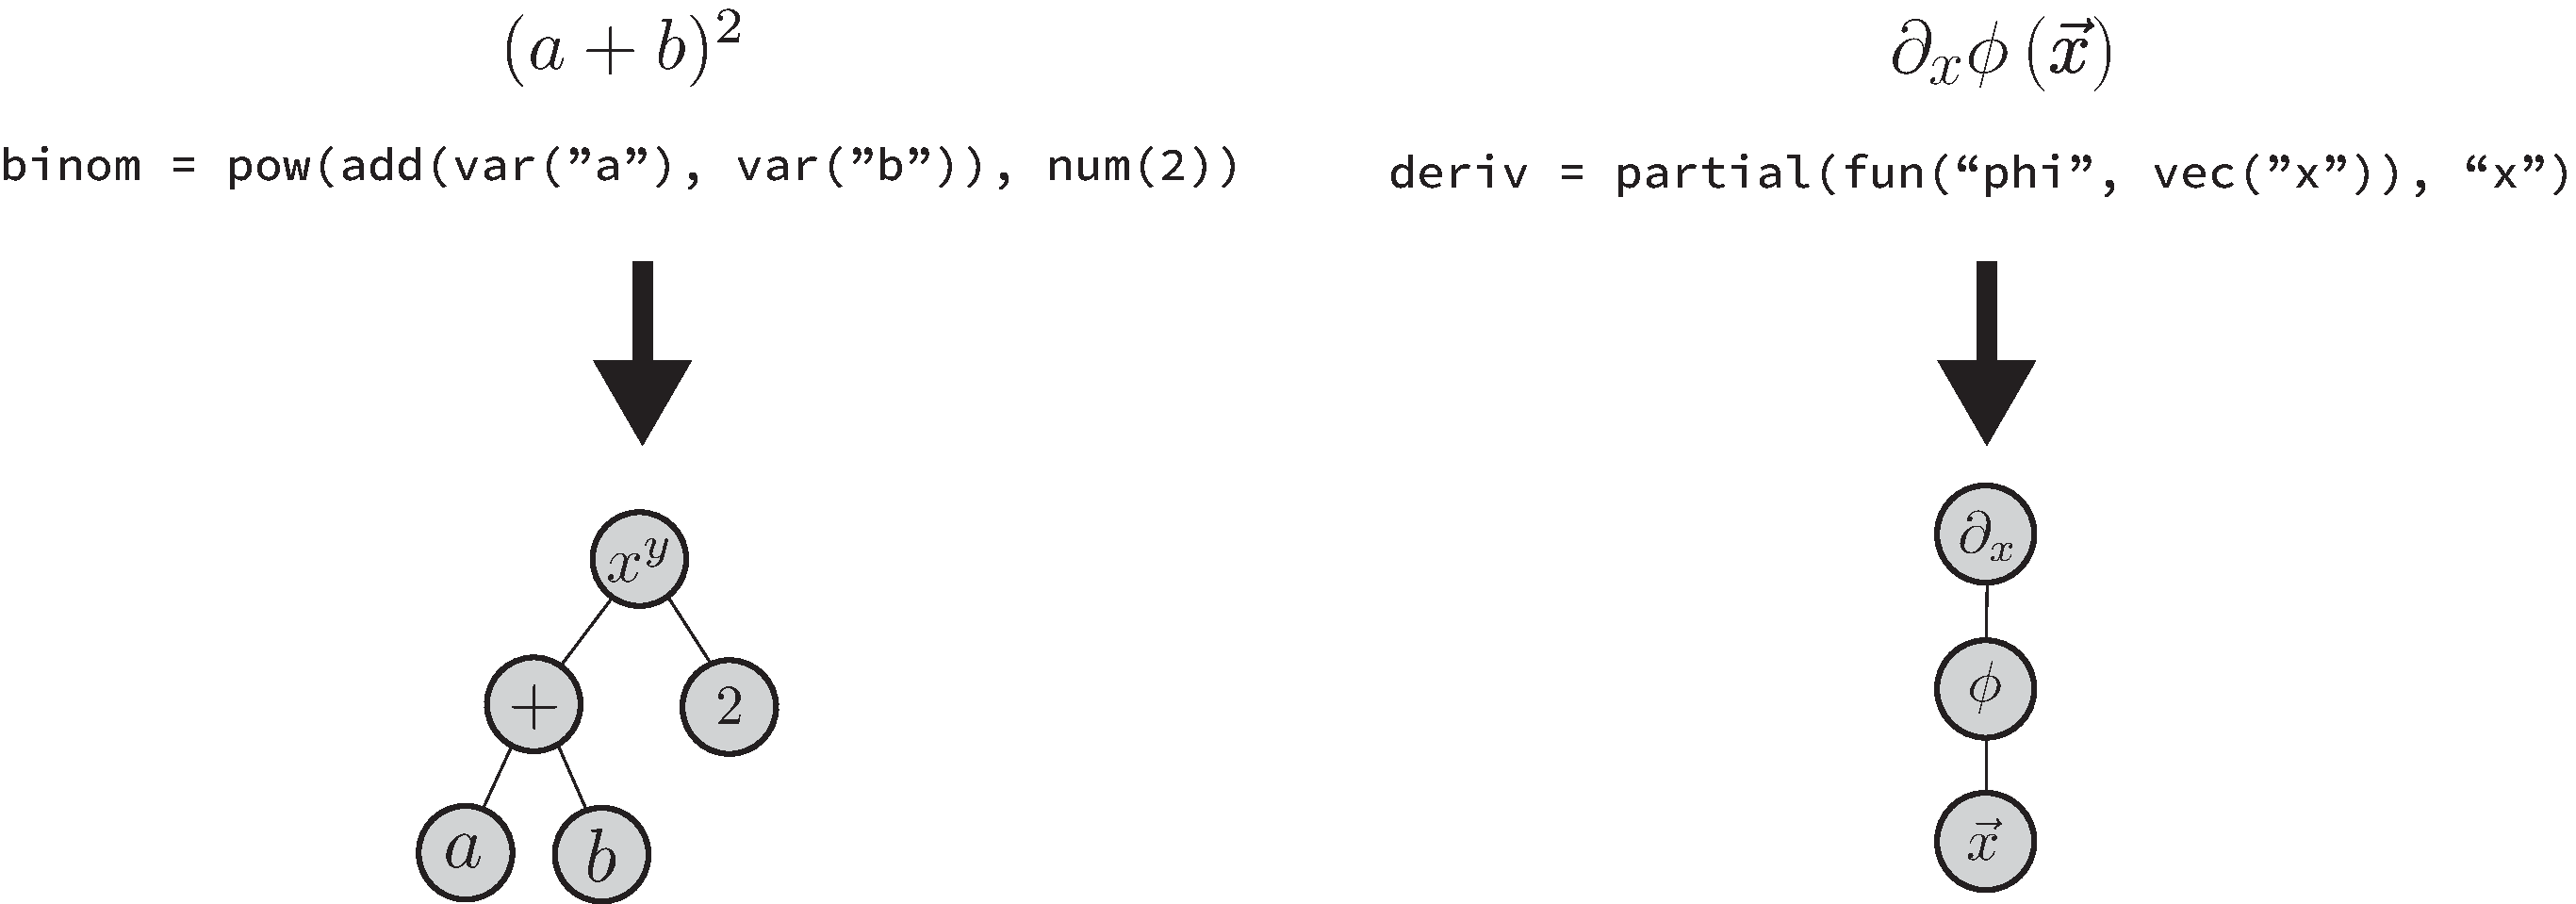
\includegraphics[width=1.0\textwidth]{04_pn_method/figures/fig_car_representation2.pdf}
\caption{An Python-API is used to create the expression tree representation for mathematical expressions.}
\label{fig:pn_math_expression_tree_generation}
\end{figure}

Manipulations of mathematical expressions, such as expansions, the application of identities, substitution, factorization or rearranging of terms can be expressed as operations on the expression tree (see figure~\ref{fig:pn_math_expression_tree_manipulation}). Section~\ref{sec:pn_stencil_gen} will assess how the spatial discretization is carried out as such an operation.
\begin{figure}[h]
\centering
%\missingfigure{image of representing binomial expansion as operation on expression tree}
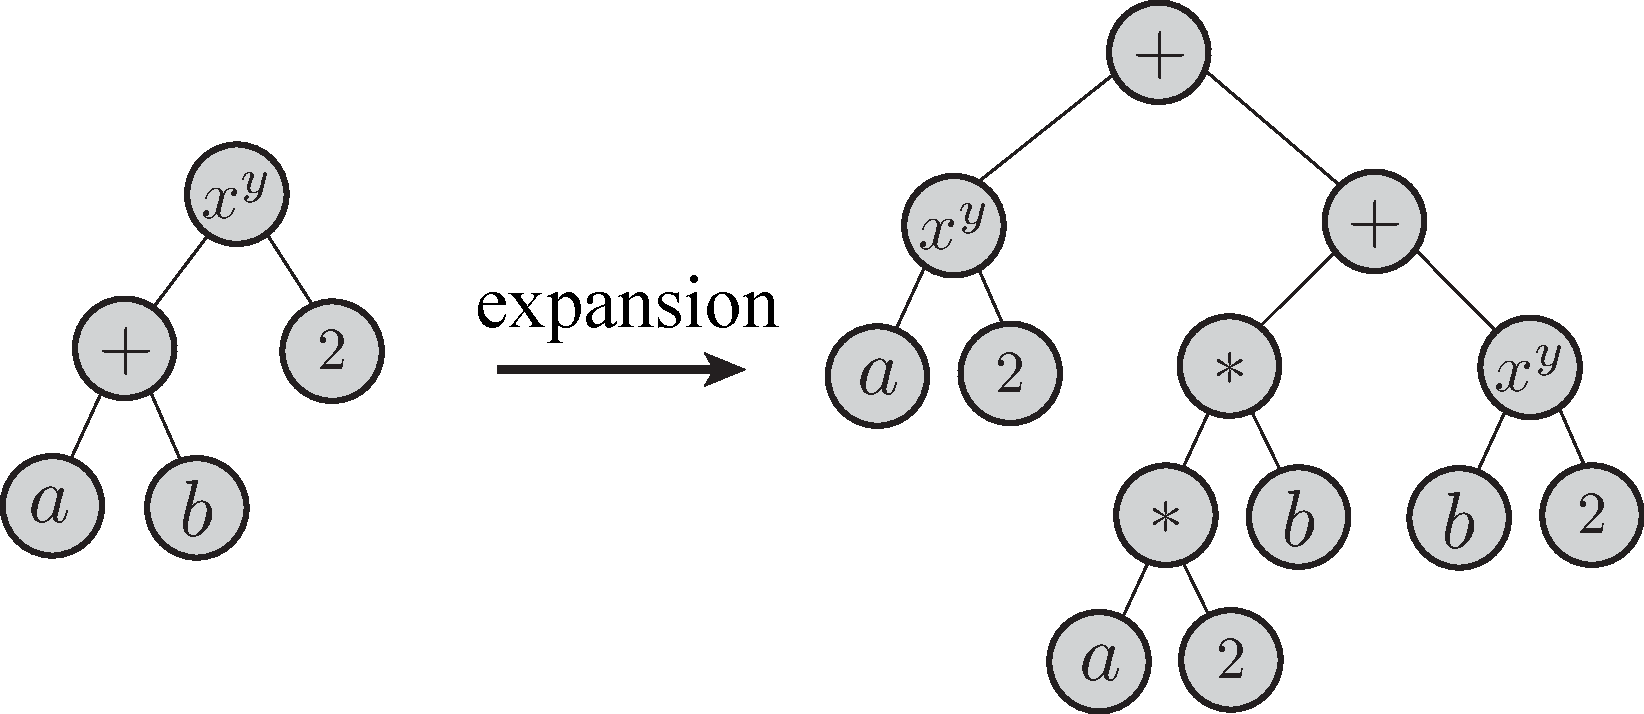
\includegraphics[width=0.7\textwidth]{04_pn_method/figures/fig_car_expansion.pdf}
\caption{Algebraic manipulations of equations are expressed as operations on the expression tree given by the computer algebra representation.}
\label{fig:pn_math_expression_tree_manipulation}
\end{figure}

\subsection{Discretization}
\label{sec:pn_stencil_gen}

After expressing the $P_N$-equations in the computer algebra representation, the spatial discretization is carried out as a manipulation step on the mathematical expression tree. This is done by parsing the tree from the root. The equation is supposed to be discretized at position $\vec{x}$, which initially coincides with the location $x_{ijk}$ in the discretized domain. This location is kept on a stack by the parser.

When a differential operator is encountered during tree parsing, the subtree representing the expression to be derived is instantiated twice according to the finite difference expression in equation~\ref{eq:pn_solver_central_difference} with appropriate weighting factors. The current position on the stack is adjusted and pushed on the stack again when descending down in the tree on each side of the central difference expression. This will produce higher order stencils for nested differential operators.
\begin{figure}[h]
\centering
%\missingfigure{image showing math expression tree for how the differential operator is being replaced with central difference. also mark the position on the stack.}
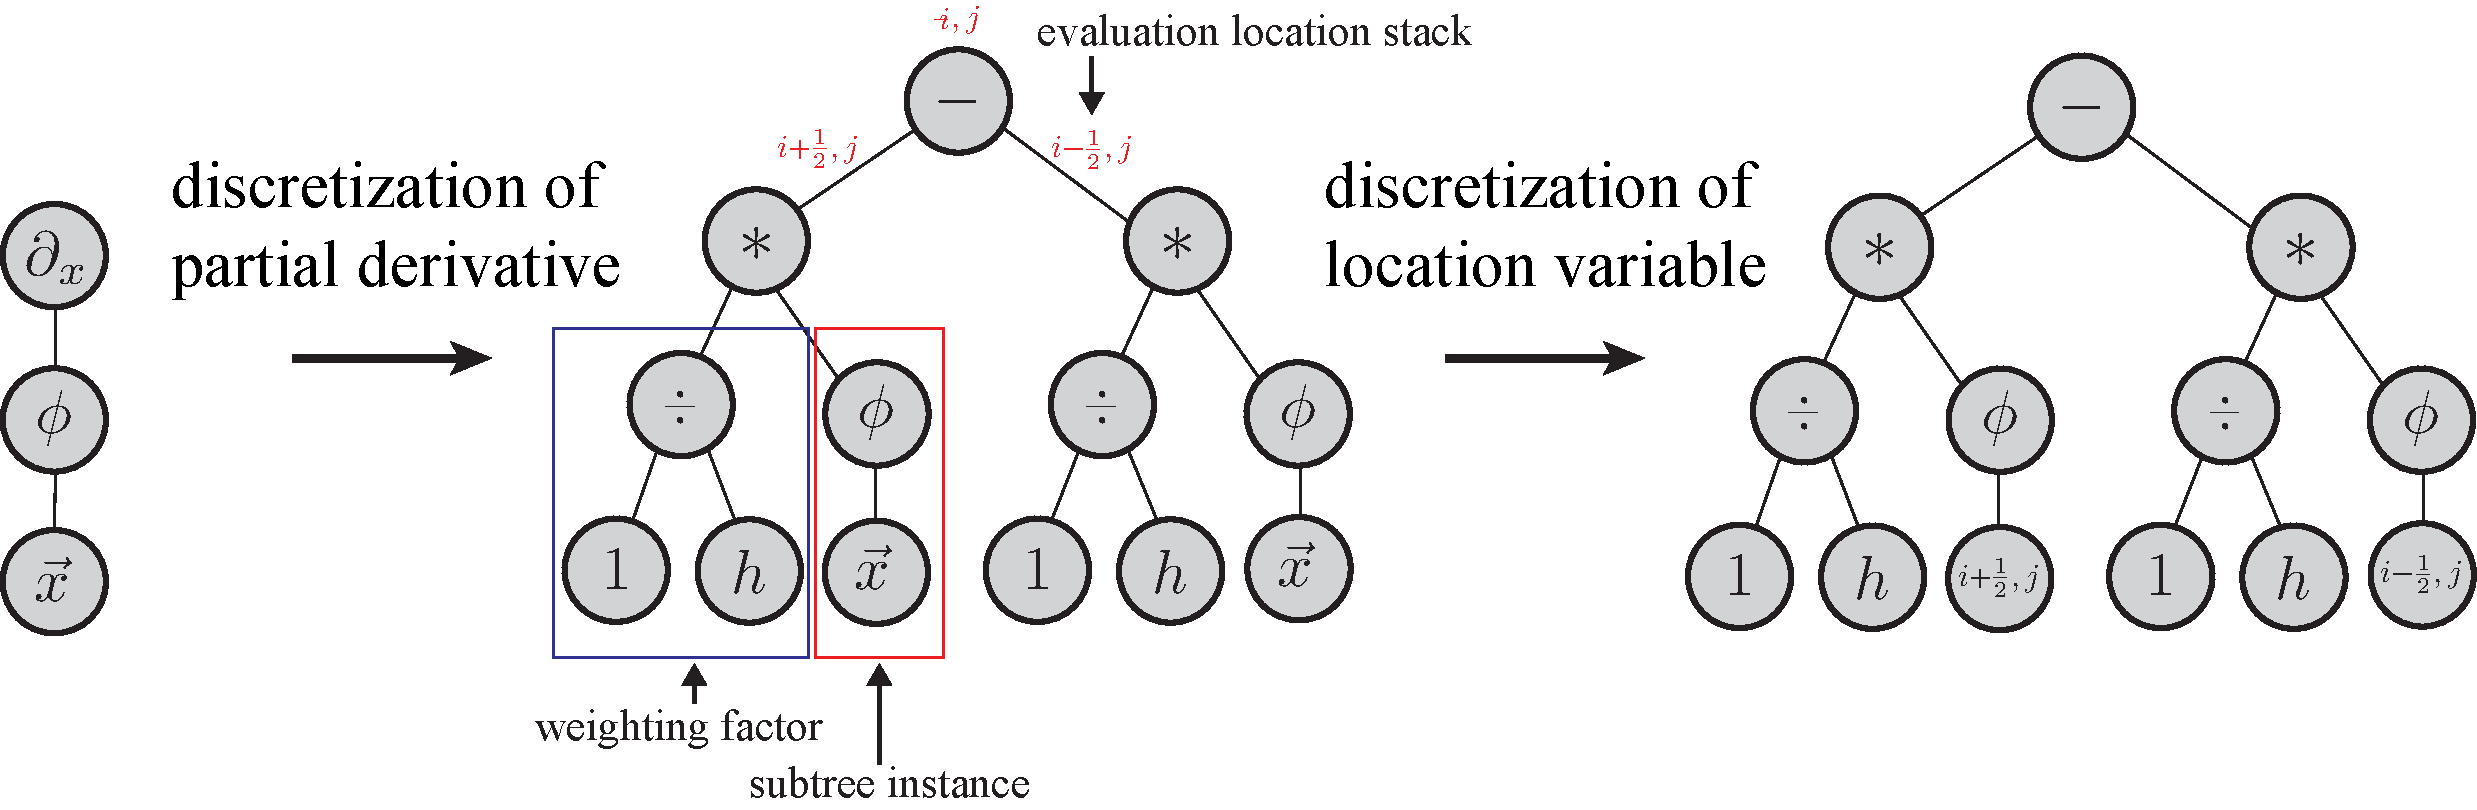
\includegraphics[width=1.0\textwidth]{04_pn_method/figures/fig_car_discretization.pdf}
\caption{Discretization is carried out as an operation on the expression tree where partial derivatives are replaced by finite difference subtrees. Continous variables are replaced by discrete counterparts, for which offsets are retrieved from a stack that is maintained during tree parsing.}
\label{fig:pn_discretization_differential}
\end{figure}

Once the parser arrives at the symbol $\vec{x}$ in the tree, it is replaced by its discrete counterpart. The top of the discrete position stack indicates where the unknown is expected to be evaluated relative to position $ijk$, at which the whole equation is being evaluated. If the position on top of the stack is the same, then the unknown at $ijk$ is used to replace $\vec{x}$ in the expression. If the unknown is expected to be evaluated at a different location than $ijk$ (due to central differences), then $\vec{x}$ is being substituted by an expression which expresses the interpolation of the unknowns from the gridpoints at which they are defined for the position on top of the stack (figure~\ref{fig:pn_discretization_interpolation}). This ensures, that the final expression only contains unknowns, for which an element in the solution vector exists. This will automatically handle the introduction of staggered grids later in section~\ref{sec:pn_staggered}.
\begin{figure}[h]
\centering
%\missingfigure{image showing interpolation.}
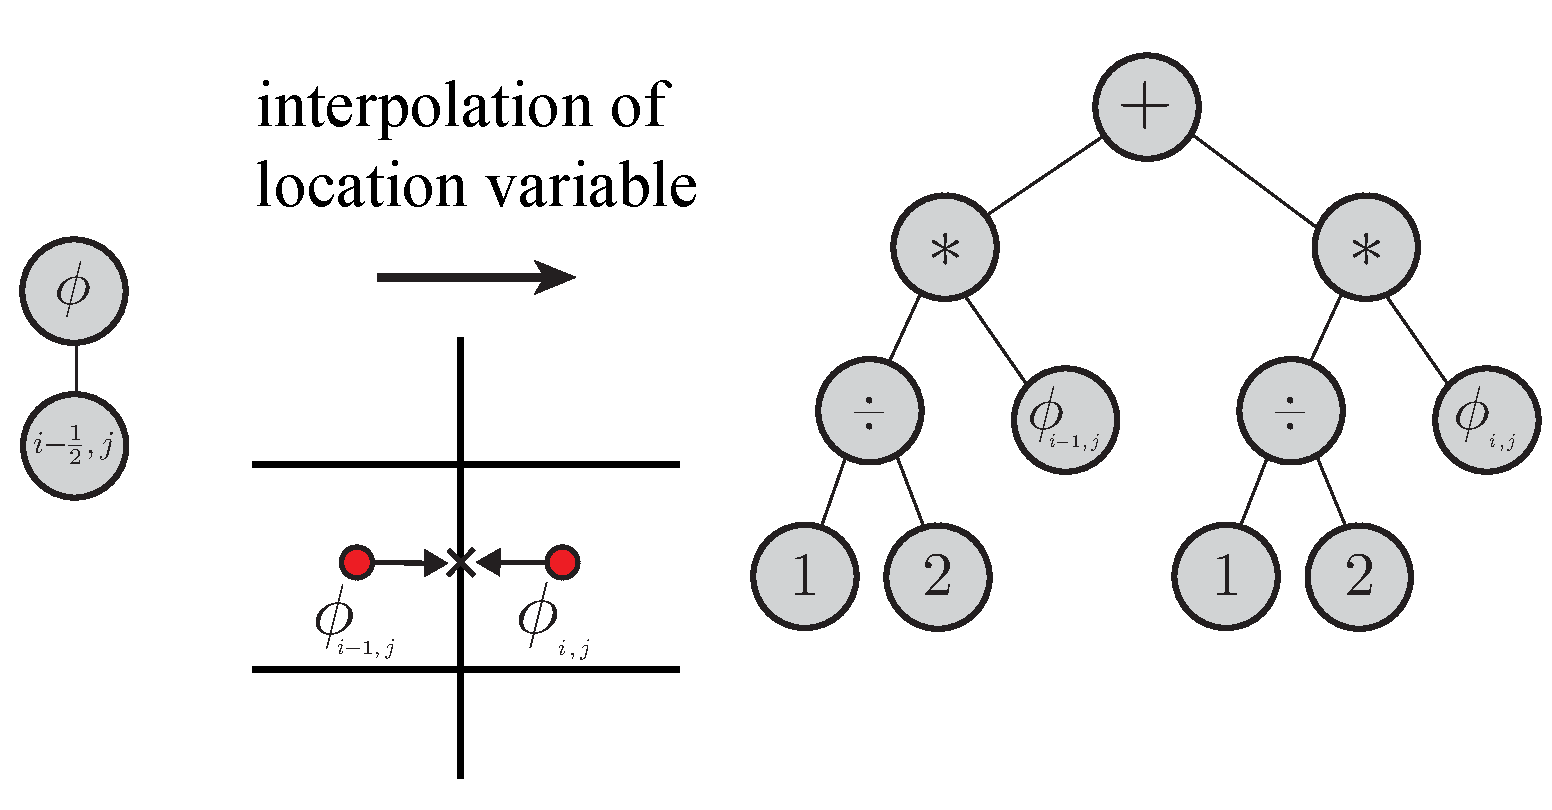
\includegraphics[width=0.7\textwidth]{04_pn_method/figures/fig_car_interpolation.pdf}
\caption{Continuous field variables are turned into discrete counterparts by replacing them with an expression subtree which realizes an interpolation.}
\label{fig:pn_discretization_interpolation}
\end{figure}

After applying the discretization to the expression tree, the equation is being factorized according to the unknowns ($\phi$ in the Laplace example). The factorization is applied as a sequence of manipulation operations to the expression tree, including application of the distributive law. A seperate step iterates over all resulting terms and merges coefficients from multiple instances of the same unknown, so that each unknown appears only once (canonical form).

\subsection{Stencil Code Generation}
\label{sec:pn_stencil_gen2}

The expression tree of the canoncial form is analyzed and rendered into stencil code. This is facilitated by different rendering frontends which allow for rendering the expression tree to latex or C++-code (see figure~\ref{fig:pn_math_expression_tree_rendering}).
\begin{figure}[h]
\centering
%\missingfigure{image showing rendering frontends for source code and latex}
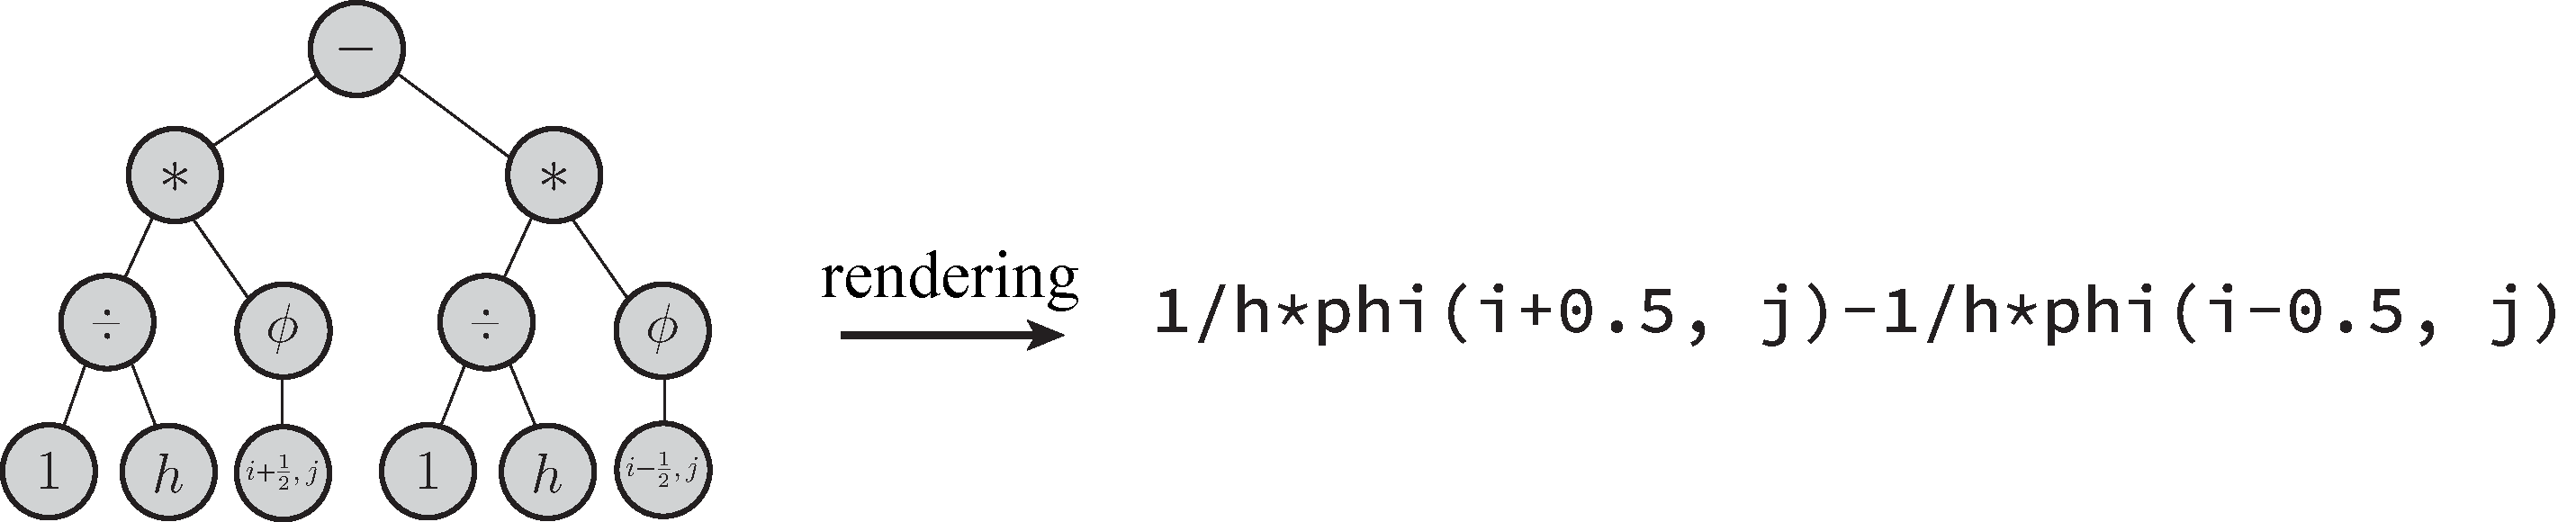
\includegraphics[width=1.0\textwidth]{04_pn_method/figures/fig_car_rendering.pdf}
\caption{Rendering frontends allow turning expression trees into source code.}
\label{fig:pn_math_expression_tree_rendering}
\end{figure}

If a term contains an unknown, then its factor expression subtree is rendered into a source code string. The symbols for voxel size and other radiative quantities are replaced by function calls into an API, which is being provided by the framework. Finally, the voxel-space coordinate associated with the unknown is used to find a discrete index into the finite difference grid, relative to the original coordinate $ijk$, at which the equation is being evaluated. This discrete index is being used to compute the column in $A$. Hence the assignment expression in the stencil code can be put together.
\begin{figure}[h]
\centering
%\missingfigure{image showing code generation from expression tree in canonical form.}
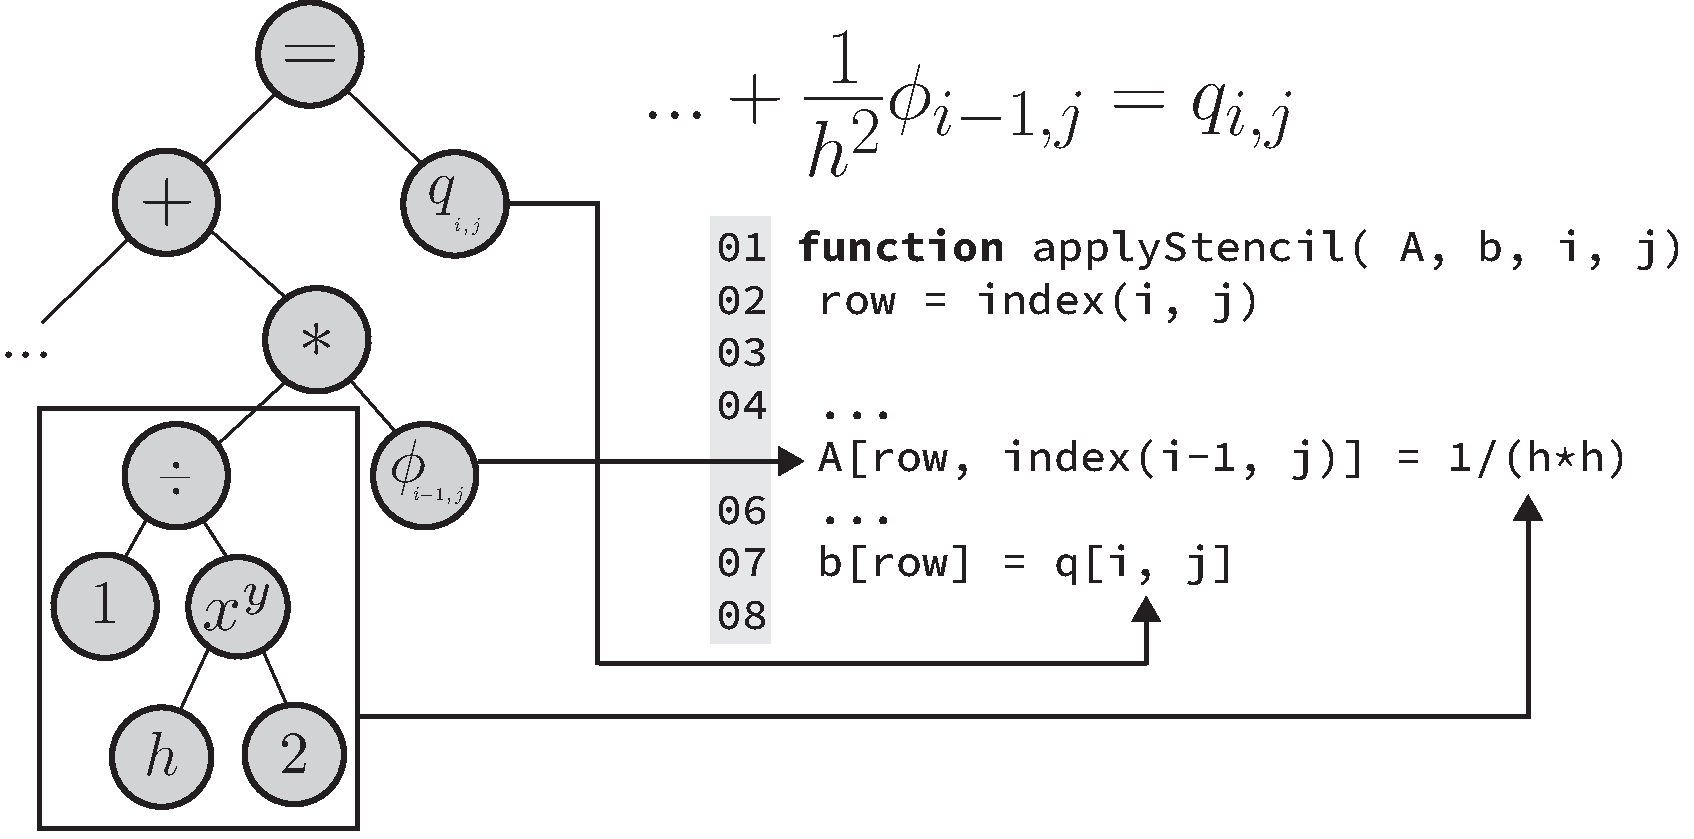
\includegraphics[width=0.6\textwidth]{04_pn_method/figures/fig_car_canonical_to_code.pdf}
\caption{The discretized equation in canonical form allows straightforward generation of stencil code from the different parts of the expression tree.}
\label{fig:pn_discretization_codegen}
\end{figure}

If the term does not contain an unknown, the whole term is rendered into a single expression, which is being assigned to the current row of the right hand side vector $\vec{b}$.

The stencil code is generated with the assumption of certain function calls being available. These are integrated into a single API which is being provided by the solver framework (figure~\ref{fig:pn_discretization_codegen_stencilAPI}). This API allows the stencil to query the current row in the system for which it is being executed, the voxelsize as well as functions for accessing discrete radiative transfer properties.
\begin{figure}[h]
\centering
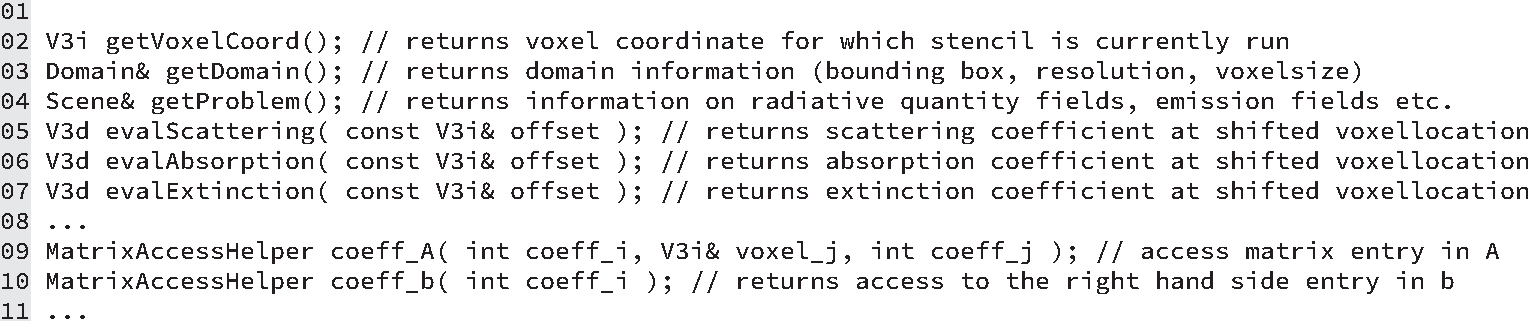
\includegraphics[width=0.95\textwidth]{04_pn_method/figures/fig_stencil_api.pdf}
%\missingfigure{image showing the stencil API}
\caption{Stencil code generation assumes an API for querying voxel fields of radiative quantities and accessing entries in coefficient matrix $A$ and right hand side $b$}
\label{fig:pn_discretization_codegen_stencilAPI}
\end{figure}


\subsection{Boundary Conditions}
\label{sec:pn_bc}

Central difference discretization will introduce references to spherical harmonics coefficients, which are outside the computational domain. Those references will be part of the stencil code, which has been generated without the notion of boundaries and boundary conditions and are handled transparently by the solver framework.

Boundary conditions define how the problem behaves directly on the boundary interface of the domain, and are an important aspect of establishing the system of linear equations. Boundary conditions can be specified without effort through the Dirichlet boundary conditions and Neumann boundary conditions, which are both supported by the system introduced in this chapter.

If $D\in\mathbb{R}^3$ defines the volume of the computational domain across which to find a solution to a partial differential equation, then $\partial D\in\mathbb{R}^3$ can be the set of points, which lie directly on the boundary of that domain. With Dirichlet boundary conditions, the value of the unknown is specified at the interface $\partial D$ directly. With Neumann boundary conditions, the behavior of the solution at the boundary is specified by giving a normal derivative of the solution. Using the Laplace example, this would be:
\begin{align*}
\text{PDE:\ \ } & \nabla^2\phi\left(\vec{x}\right) = q\left(\vec{x}\right)
&
\\
\\
\text{Dirichlet BC:\ \ } & \phi\left(\vec{x}\right) = f\left(\vec{x}\right)
&\forall \vec{x}\in\partial D
\\
\\
\text{Neumann BC:\ \ } & \frac{\partial\phi\left(\vec{x}\right)}{\partial\vec{n}} = g\left(\vec{x}\right)
&\forall \vec{x}\in\partial D
\end{align*}
In most applications for computer graphics, a value of zero for either Dirichlet or Neumann boundaries is adequate and is handled by the system through remapping the index: Considering the first term of the discretized Laplace equation in equation~\ref{eq:pn_laplace_canonical_form}, the result is the following assignment within the stencil code:
\begin{align}
A[\mathrm{index}(i,j), \mathrm{index}(i+1, j)] = 1.0/(h_x*h_x);
\end{align}
The function call $index(i+1, j)$ will not be able to produce a valid column index into the coefficient matrix $A$ for voxels adjacent to the boundary, because the unknown $\phi$ has no discrete element in the solution vector voxels outside the domain. If the value of $\phi$ on the boundary is zero, then the unknown on the boundary voxel would be zero and its coefficient would not matter. Therefore, the simplest solution is to ignore the coefficient not writing anything into the matrix $A$. This equates to matrix $A$ being zero outside the computation domain.

In the solver framework, this is implemented by overloading the assignment operator. If the target coefficient of the assignment belongs to a boundary voxel and Dirichlet boundary conditions are enabled, then the assignment is simply ignored and no change to the system matrix $A$ is done.

\begin{figure}[h]
\centering
%\missingfigure{image: boundary voxels and dirichlet boundary condition. location of the boundary interface.maybe an arrow indicating the access of the stencil.show assignment and arrow to boundary voxel coefficient. then arrow to nil.also visualize the boundary surface.}
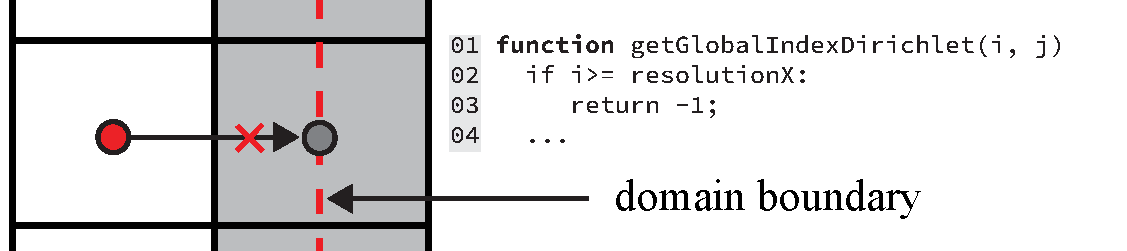
\includegraphics[width=0.8\textwidth]{04_pn_method/figures/fig_bc_dirichlet.pdf}
\caption{Dirichlet boundary conditions with zero value are modelled by ignoring coefficient assignments to boundary voxels.}
\label{fig:pn_bc_dirichlet}
\end{figure}

With Neumann boundary conditions, the derivative is specified at the boundary. Since the derivative is found using central differences between two adjacent voxels, the boundary condition is controlled by how the coefficient at the voxel near the boundary relates to its adjacent coefficient at the boundary voxel. In the simplest case, the derivative is set to zero, in which the boundary voxel coefficient needs to be identical with its adjacent voxel inside
\begin{align*}
\partial\phi=0\quad\forall\phi\in\partial D
\implies
\frac{\phi_{i+1,j}-\phi_{i,j}}{h_x} = 0
\implies
\phi_{i+1,j}=\phi_{i,j}
\ .
\end{align*}
In the case of adjacent coefficients being equal across the boundary interface, a coefficient $b$ assigned to the boundary $\phi_{i+1,j}$ can be added to the adjacent unknown inside the domain resulting in:
\begin{align}
a\phi_{i,j} + b\phi_{i+1,j} = \left(a+b\right)\phi_{i,j}
\quad \text{with}\quad \phi_{i+1,j}=\phi_{i,j}
\end{align}

In the solver framework, this is implemented by index remapping. If the target coefficient of the assignment belongs to a boundary voxel and Neumann boundary conditions are enabled, then the index function returns the index of the adjacent voxel inside the domain.

\begin{figure}[h]
\centering
%\missingfigure{image showing neumann boundary conditions and index bending. also visualize the boundary surface.}
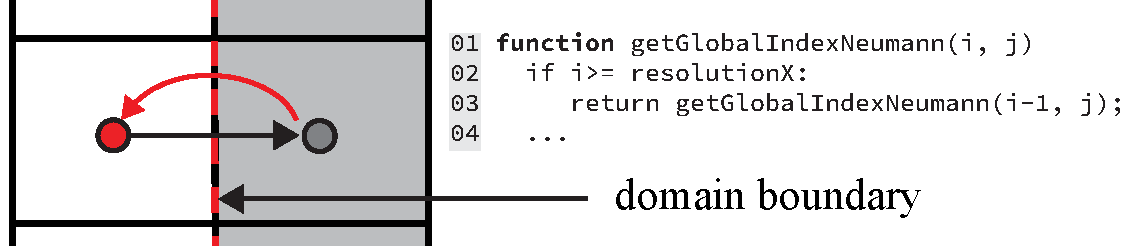
\includegraphics[width=0.8\textwidth]{04_pn_method/figures/fig_bc_neumann.pdf}
\caption{Neumann boundary conditions with zero value are modelled by remapping indices towards the adjacent inner voxel when assigning coefficients.}
\label{fig:pn_bc_neumann}
\end{figure}

Note how the choice and implementation of the boundary condition has an effect on where the effective boundary interface of the domain is located. With Dirichlet boundary conditions, the interface is directly located at the voxel centers of boundary voxels, while with Neumann boundary conditions, the interface is located at directly between the boundary voxels and inner voxels (figure~\ref{fig:pn_bc_dirichlet} and figure~\ref{fig:pn_bc_neumann}).

\subsection{Solver Framework}
\label{sec:pn_framework}

The stencil code is the result of the automated discretization step, which is carried out on the computer algebra representation and rendered into source code. The resulting stencil code is compiled and linked with a solver framework, which runs it to propagate the system matrix $A$ and right hand side vector $\vec{b}$. By rendering the tree to a different representation and assuming a different API used by the stencil code, different solver frameworks can be supported.
Therefore, the details about the surrounding framework are not relevant to the method in this thesis. In this section, however, an outline of the framework, which was implemented as part of this thesis will be given.
\begin{figure}[h]
\centering
%\missingfigure{class diagram of solver framework, including stencil, stencil api, voxelmanager, fields and pnsystem}
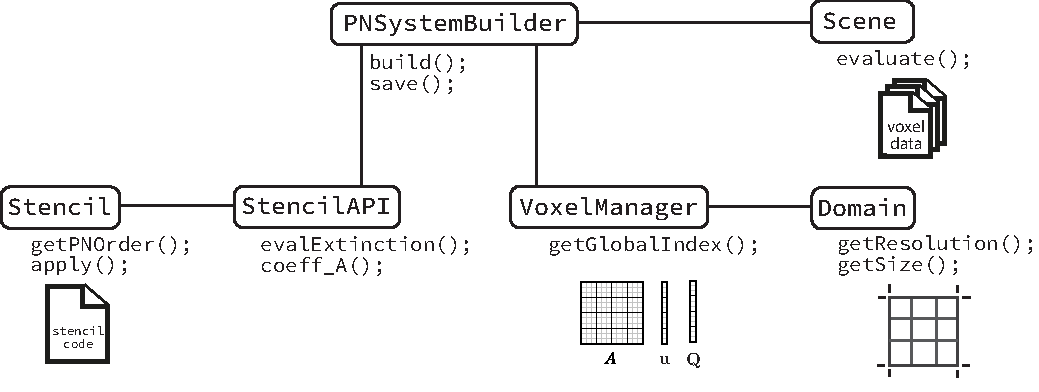
\includegraphics[width=0.95\textwidth]{04_pn_method/figures/fig_pn_solver_architecture.pdf}
\caption{High level overview over the $P_N$-solver architecture.}
\label{fig:pn_classes}
\end{figure}

The \emph{Stencil} class is the key structure around which the system is designed, and which serves as a wrapper around the generated stencil code. It specifies the dimension (two- or threedimensional) and the truncation order $N$, as these parameters are being decided during stencil code generation. The \emph{Stencil} class also indirectly specifies the number of spherical harmonics coefficients per voxel. It further specifies the placement of each spherical harmonics coefficient within the voxel. This will become important when staggered grids are introduced. The stencil specifies the highest order of any derivative operator, which was found during discretization. This affects the number of layers of boundary voxels around the computational domain. Finally, the \emph{Stencil} class has an apply function, which takes the reference to a \emph{StencilAPI} object as an input and runs the generated stencil code that uses that API to propagate the system matrix $A$ and right hand side vector $\vec{b}$.

The \emph{StencilAPI} class serves as the single interface between the generated stencil code and the surrounding parts of the framework. Figure~\ref{fig:pn_discretization_codegen_stencilAPI} gives an overview of the different query functions offered by the API. Essential are functions for mapping between coordinate spaces, such as world-space, voxel-space, discrete grid coordinates $ijk$ and linear indices into the solution vector. Further, those functions allow querying radiative transfer quantities, such as extinction coefficient or phase function spherical harmonics coefficients at world space positions. Both groups of functions will make use of a reference to a \emph{VoxelManager} and a \emph{Scene} class, respectively.

The \emph{Scene} class contains all inputs required to specify the problem to be solved. A \emph{Domain} object describes the extent of the computational domain in world-space, as well as the resolution of the finite difference grid. Further attached are references to abstract \emph{Field} interfaces, which allow querying scalar or vector fields at arbitrary worldspace positions for extinction coefficient, albedo, and the spherical harmonics coefficients of phase function and emission field. This is the place where the problem description is provided as input to the system. Different implementations of these abstract interfaces can be used, such as \emph{Constant} fields or \emph{VoxelGrid} fields. This follows the idea of resolution independent volumes introduced by Tessendorf et al.~\cite{Tessendorf11}.

The resolution of the finite difference grid provided by the \emph{Domain} class and the number of spherical harmonics coefficients by the \emph{Stencil} class, impose the layout of the voxel grid on the system. The \emph{Stencil} class gives the highest order of the derivation operator found during discretization, and with that drives the number of layers of boundary voxels. The final system of linear equations has to be a single column solution vector with a coefficient matrix of compatible dimensions. Since the computational domain is discretized using grid coordinates $ijk$, a mapping from three-dimensional coordinates $ijk$ and spherical harmonics coefficient index $c$ to a linear global index needs to be provided. This task becomes more involved, when staggered grids are introduced. This bookkeeping of interior and boundary voxels and their contained spherical harmonics coefficients is performed by the \emph{VoxelManager} class. This class is initialized with the information about the grid resolution by the \emph{Domain}, number of boundary voxel layers, number of coefficients, and the position of each coefficient on the grid by the \emph{Stencil} class. It manages the memory and mapping from multidimensional grid indices to linear indices within the global system.

Finally, the \emph{PNSystemBuilder} class is the structure, which brings the different parts together. It is initialized wit the \emph{Scene} class and the \emph{Stencil} class. Both are provided by the client code and are used during initialization to set up the \emph{VoxelManager}, which provides the layout and setup for the solution vector $\vec{u}$, right hand side vector $\vec{b}$ and system matrix $A$. The purpose of the \emph{PNSystemBuilder} class is to build the system matrix $A$ and right hand side vector $\vec{b}$ and return both to client code. This is done by calling the \emph{build} function on the object.

The \emph{build} function iterates over all voxels. For each voxel, the \emph{StencilAPI} object is set up with the correct indices and data pointers and passed as an argument to a call of the \emph{apply} function of the \emph{Stencil} class. As explained in section~\ref{sec:pn_stencil_gen}, the stencil code will make appropriate calls to the \emph{StencilAPI} object, which will propagate the system matrix $A$ and right hand side vector $\vec{b}$ with the correct values for the row, corresponding to the current voxel in the cycle of the \emph{build} function. The system is fully propagated after the stencil has been executed for every voxel. Separate functions of the \emph{PNSystemBuilder} class allow querying the system matrix $A$ and right hand side vector $\vec{b}$ after those have been build.

\subsection{Staggered Grids}
\label{sec:pn_staggered}

In figure~\ref{fig:pn_staggered_grid_problems}\subref{fig:pn_collocated_grid_artefacts}, preliminary results for the two-dimensional checkerboard problem are shown, a popular reference problem for deterministic methods (section~\ref{sec:pn_results}). As seen in the figure, it suffers from severe artifacts, showing an oscillating structure. The cause for these artifacts is a known problem for partial differential equations, which have different quantities influencing each other at the same spatial grid locations. The problem is visualized in figure~\ref{fig:pn_staggered_grid_problems}\subref{fig:pn_staggered_grid_idea}, using a simple one-dimensional grid as an example. Shown is a simple setup with two variables, which are located at the same grid points, referred to as collocated grids. The variable $\beta$ depends on the derivative of $\alpha$. Due to central difference discretization, two different solutions that are decoupled from each other can emerge. These solutions are interleaved in an oscillating pattern throughout the grid as shown in the upper part of the figure.

\begin{figure}[h]
\centering
\begin{subfigure}[t]{0.49\columnwidth}
\centering
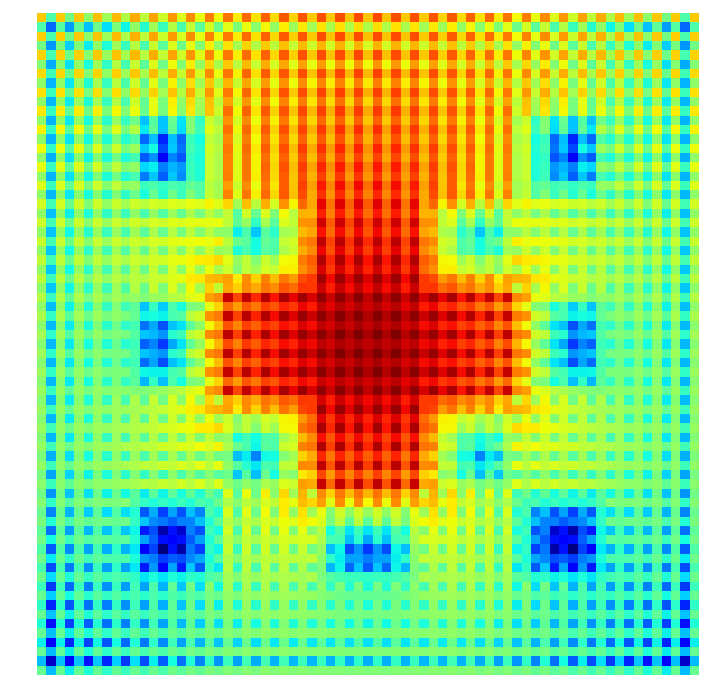
\includegraphics[width=\columnwidth]{04_pn_method/results/checkerboard2d_p1_collocated.png}
%\missingfigure{2d collocated solution with artefacts}
\caption{$P_1$-solution of the checkerboard problem using collocated discretization grid.}
\label{fig:pn_collocated_grid_artefacts}
\end{subfigure}%
\hspace{0.01\columnwidth}
\begin{subfigure}[t]{0.49\columnwidth}
\centering
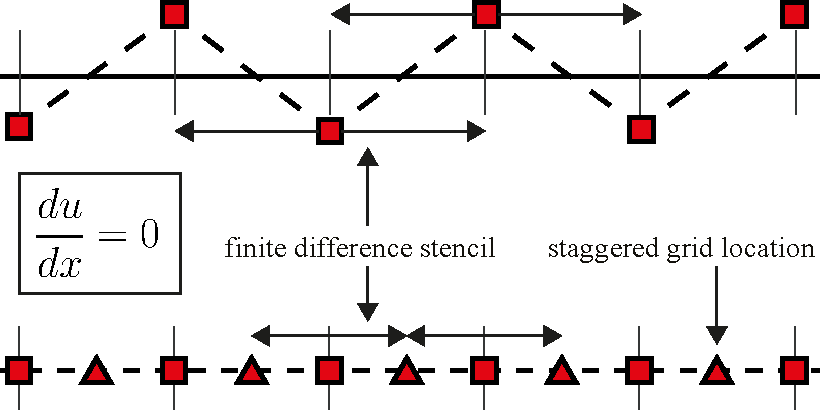
\includegraphics[width=\columnwidth]{04_pn_method/figures/fig_staggered_grid_1d_example.pdf}
%\missingfigure{1d schematic view of staggered grid idea, showing the problem with collocated grids}
\caption{Example showing the problem with finite differences producing a false solution (top) and its treatment with staggering (bottom).}
\label{fig:pn_staggered_grid_idea}
\end{subfigure}%
%\vspace{-0.2in}
\caption{Artefacts in the solution (left) due to shortcomings of collocated grid locations. These are addressed using staggered grids (exemplified right).}
\label{fig:pn_staggered_grid_problems}
\end{figure}

The solution to this problem is to offset the coefficients $\alpha$ and $\beta$ from each other spatially. This configuration is called staggered grids. As visualized in figure~\ref{fig:pn_staggered_grid_problems}\subref{fig:pn_staggered_grid_idea} bottom, setting up the coefficients in that way prevents decoupling and results in a single coherent solution throughout the grid. A similar staggering of the interdependent variables is required for the $P_N$-solver to produce correct results.

The staggered grid locations are found by subdividing the original grid into a finer grid of double resolution. The locations are at the grid points of that finer grid. In terms of the original grid, these are located at the voxel centers, the center of the voxel faces between adjacent voxels, the center of voxel edges and at voxel corners as shown in figure~\ref{fig:staggered_grid}.
\begin{figure}[h]
\centering
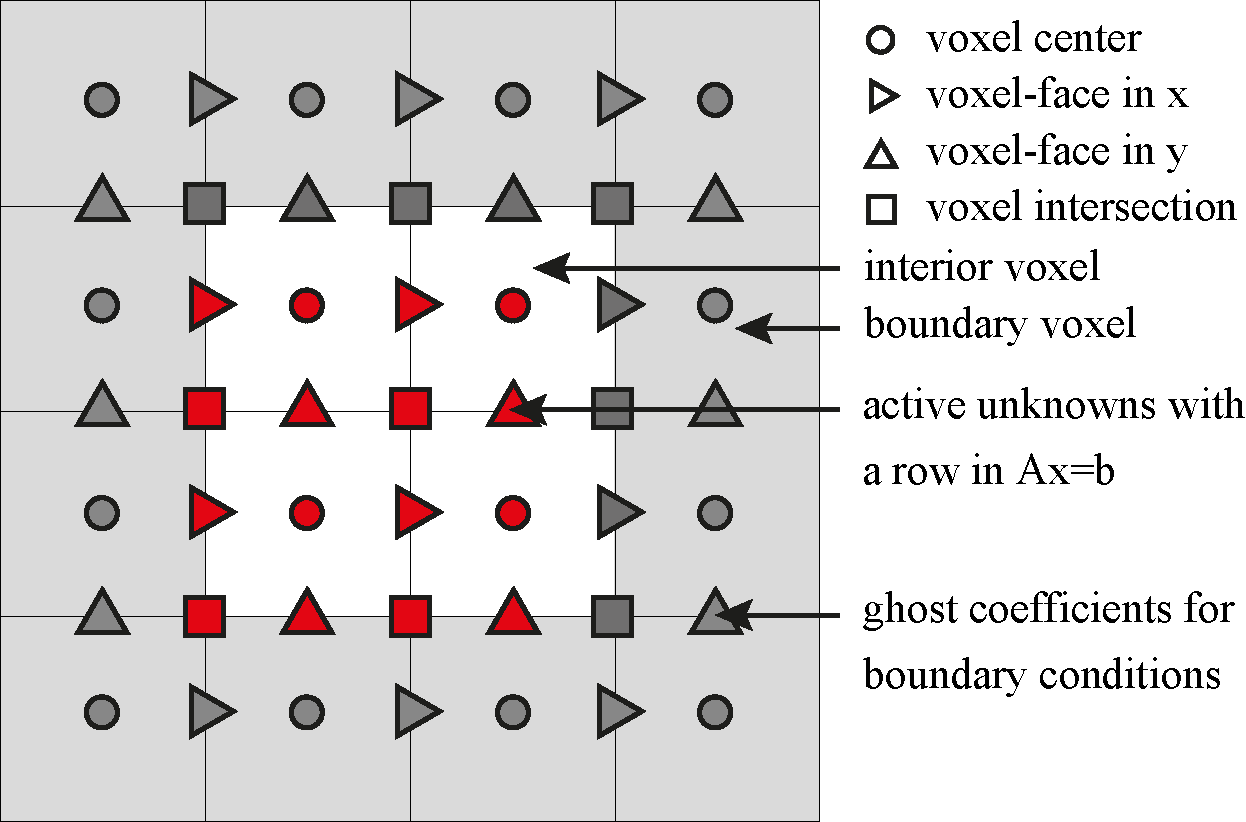
\includegraphics[width=0.65\textwidth]{04_pn_method/figures/fig_staggered_grid.pdf}
\caption{Staggered grid configuration in 2d. Extending the concept to 3d is straightforward.}
\label{fig:staggered_grid}
\end{figure}

With a staggered grid configuration, the question is which unknowns (the spherical harmonics coefficients) are placed at which staggered grid location. Seibold et al.~\cite{Seibold14} analysed the structure of the transport term and found that its discretization matrix relates coefficients to their derivatives in a very particular structure after converting the matrix to real-valued spherical harmonics. If coefficients are located on the staggered grid according to this structure, hence no interpolation is required when evaluating central differences of the stored coefficients (see figure~\ref{fig:staggered_grid_placement}).

Assuming this structure, the unknown locations are found by the following algorithm: First the zero coefficient is placed at the voxel center. Then all coefficients are found, which depend on derivatives of the zero coefficient. These coefficients are placed according to the central difference offsets. Following this, the coefficients are found, which depend on derivatives of the recently placed coefficients. The central difference offsets are used anew to find their new location. The particular structure of discretization matrix of the transport term in the real-valued $P_N$-equations is what allows placing the coefficients without any conflicts. 
\begin{figure}[h]
\centering
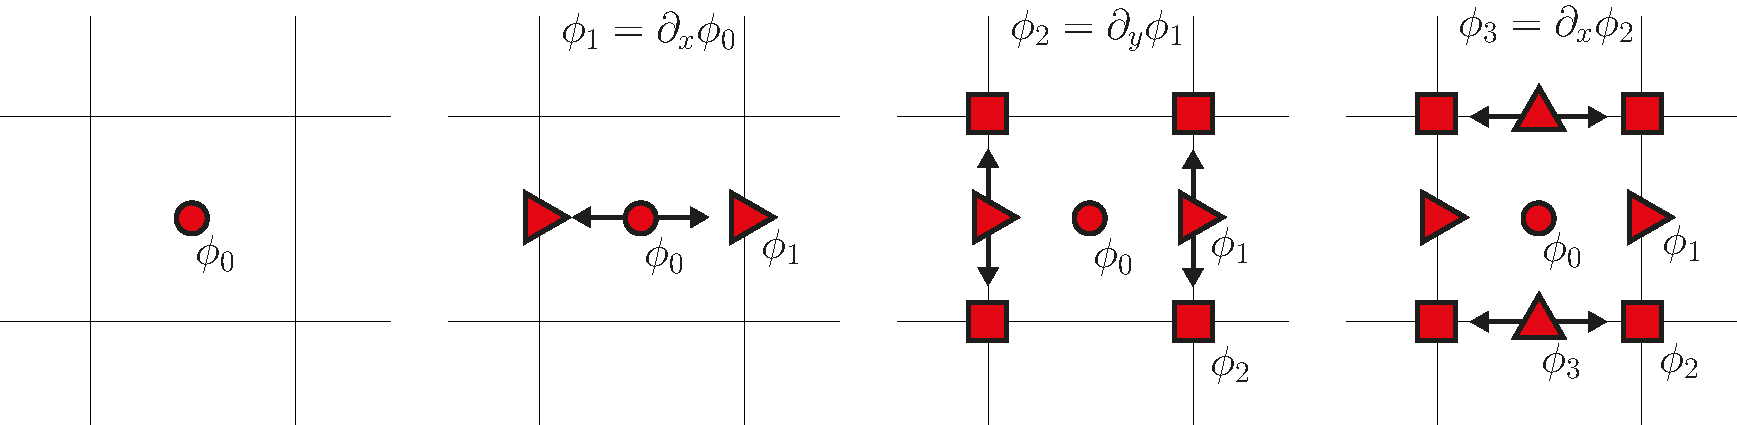
\includegraphics[width=0.95\textwidth]{04_pn_method/figures/fig_staggered_grid_finding_locations.pdf}
\caption{The process of finding staggered grid locations for unknowns $\phi_i$. The $P_N$-equations relate the unknowns through spatial derivatives, which imply an order on the finite difference grid. The first unknown is placed at the voxel center and the remaining unknown locations are found by following the spatial derivatives through the equations.}
\label{fig:staggered_grid_placement}
\end{figure}

It is important to realize that each equation in the system of linear equations relates a particular coefficient with spherical harmonics indices $l,m$ in a particular voxel within the finite difference grid to other coefficients at the same or adjacent voxels (due to derivatives). Therefore, the equation associated with a particular spherical harmonics index $l,m$ within the $P_N$-equations, is implicitly defined at the location of the spherical harmonics coefficient with the same $l,m$ index. Due to staggering, the equations are consequently defined at different locations. This has a paramount consequence for the spatial discretization step during stencil code generation.

In section~\ref{sec:pn_stencil_gen} the spatial discretization was carried out as a manipulation on the expression tree representing the $P_N$-equations. This manipulation step traversed the tree and replaced the continuous spatial variable $\vec{x}$ by its discrete counterpart $x_{ijk}$. During traversal, a stack was used to keep track of the current location which would change due to shifts from central difference discretizations of differential operators within the expression tree. This stack was initialized with the reference position $x_{ijk}$, which would refer to the voxel center. This was correct, as all coefficients and equations were collocated at this position. With staggered grids, the equations are to be evaluated at the grid location implied by the position of the respective spherical harmonics coefficient with index $l,m$. Therefore, to account for staggered grids, the position stack needs to be initialized with the staggered grid location of the $l,m$-equation, which is being discretized.

The discretization step will replace the evaluation of a coefficient at a particular location, with an interpolation of that coefficient from the surrounding grid locations at which it is defined (figure~\ref{fig:pn_discretization_interpolation}). This approach will handle the staggering naturally.

Staggering spherical harmonics coefficients also makes handling boundary conditions more involved. With collocated grids, it is straightforward to identify boundary voxels and voxels in the computational domain. Each voxel in the computational domain contributes the same number of unknowns to the system. With staggered grids, some boundary voxels will have a subset of their unknowns that lie directly on the boundary. Without changes to the system, this will imply a shifted boundary interface and introduce an asymmetry. Coefficients, which are located on the boundary, will be unknowns and part of the solution vector on one side and subject to boundary conditions on the other side (figure~\ref{fig:pn_staggered_grid_unhandled_bc}~\subref{fig:pn_staggering_asymmetry_bc}). This creates different boundary conditions on opposite sides of the problem domain and causes an asymmetry in the solution for symmetric problems (figure~\ref{fig:pn_staggered_grid_unhandled_bc}~\subref{fig:pn_staggering_asymmetry_bc_checkerboard}).
\begin{figure}[h]
\begin{subfigure}[t]{0.48\columnwidth}
\hspace{0.5in}
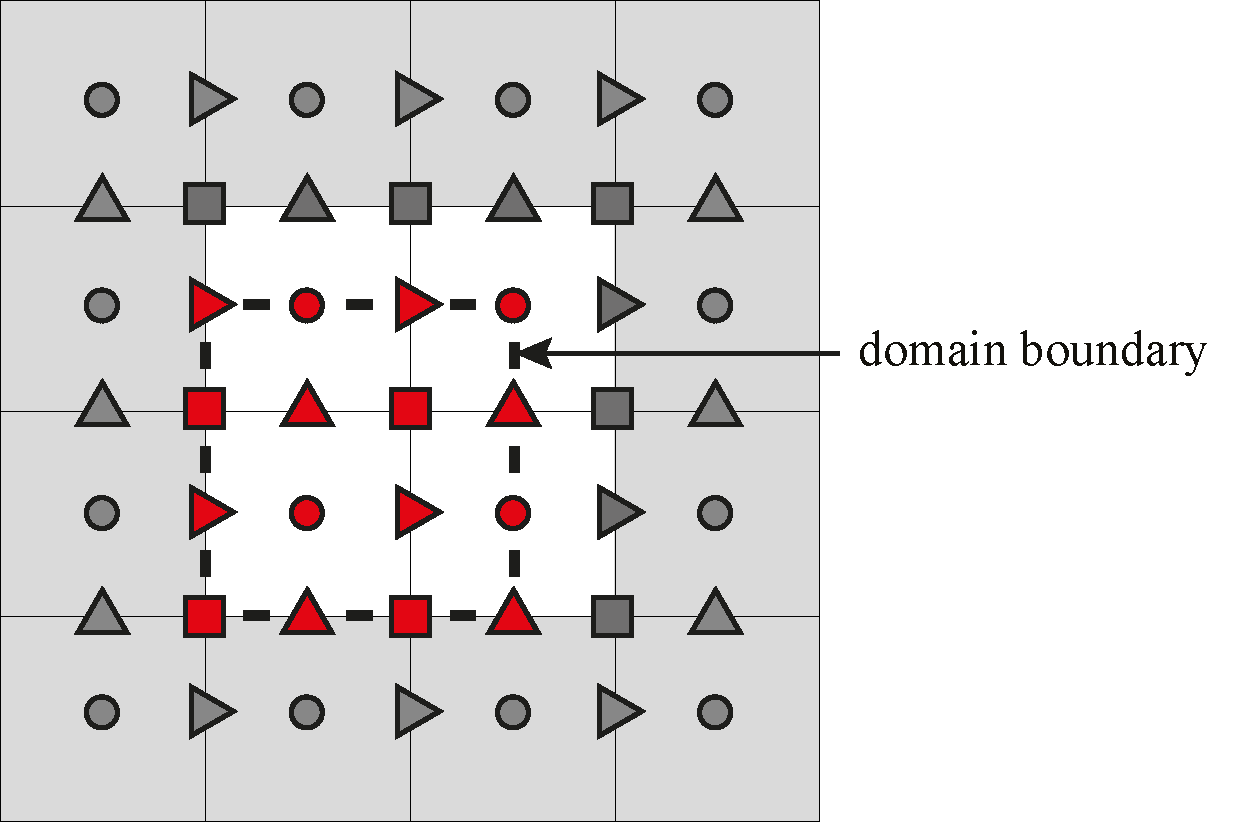
\includegraphics[width=1\textwidth]{04_pn_method/figures/fig_staggered_grid_domain_boundary_wrong.pdf}
\caption{Per voxel staggered grid locations.}
\label{fig:pn_staggering_asymmetry_bc}
\end{subfigure}
\hspace{0.01\columnwidth}
\begin{subfigure}[t]{0.48\columnwidth}
\centering
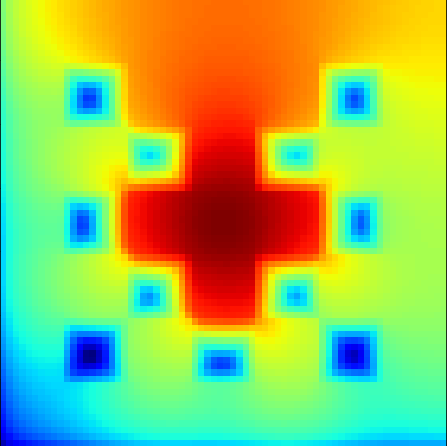
\includegraphics[width=0.66\columnwidth]{04_pn_method/results/p1_staggered_grid_asymmetric_bc.png}
\caption{$P_1$-solution.}
\label{fig:pn_staggering_asymmetry_bc_checkerboard}
\end{subfigure}
\caption{Dealing with staggered grid locations per voxel (left) implies a boundary interface which produces asymmetric results as seen for the solution of the checkerboard problem (right).}
\label{fig:pn_staggered_grid_unhandled_bc}
\end{figure}

The solution is to introduce additional unknowns to the system for every coefficient which is located in a boundary voxel as shown in figure~\ref{fig:pn_staggered_grid_handled_bc}\subref{fig:pn_staggering_correct_bc}. This will correct the location of the boundary interface and allows the same boundary conditions on opposite sides of the computational domain.
\begin{figure}[h]
\centering
\begin{subfigure}[t]{0.49\columnwidth}
\centering
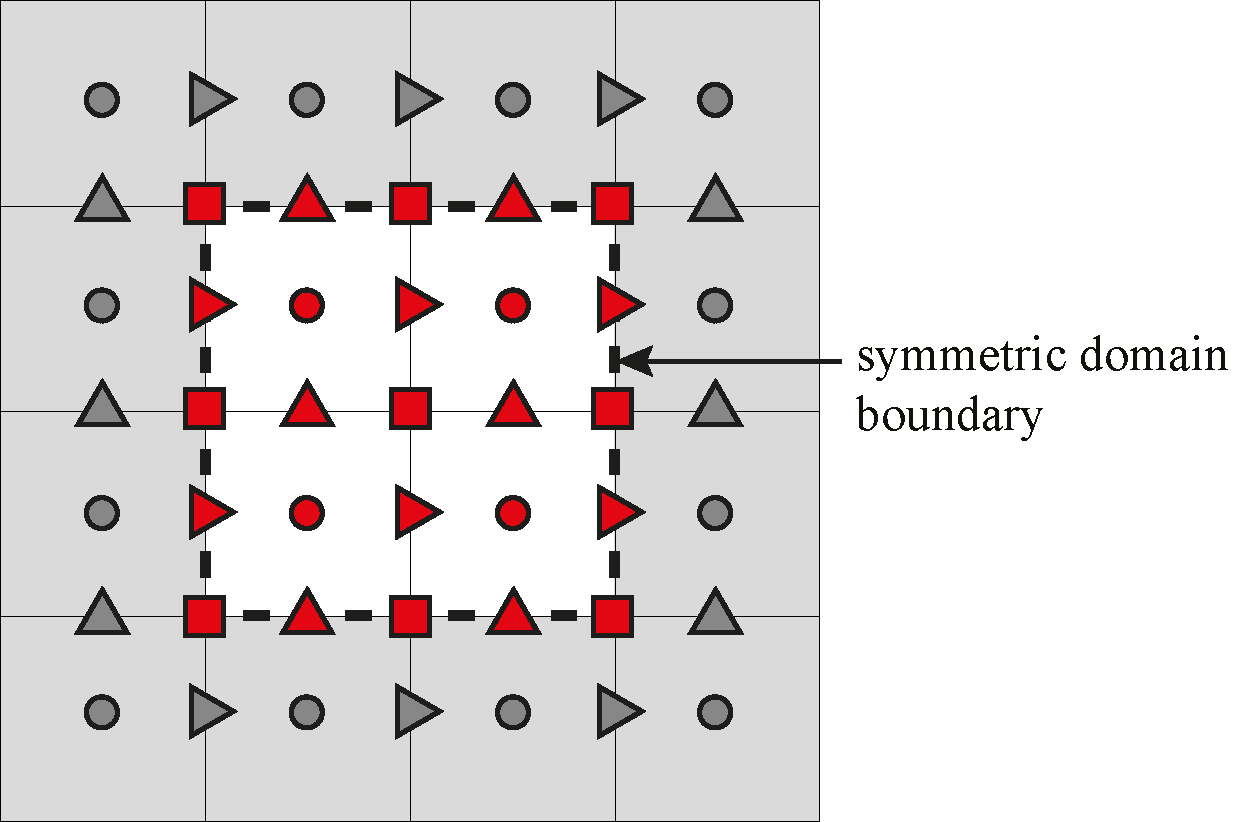
\includegraphics[width=1\textwidth]{04_pn_method/figures/fig_staggered_grid_domain_boundary_corrected.pdf}
\caption{Adjusted placement of staggered grid coefficients.}
\label{fig:pn_staggering_correct_bc}
\end{subfigure}
\hspace{0.01\columnwidth}
\begin{subfigure}[t]{0.34\columnwidth}
\centering
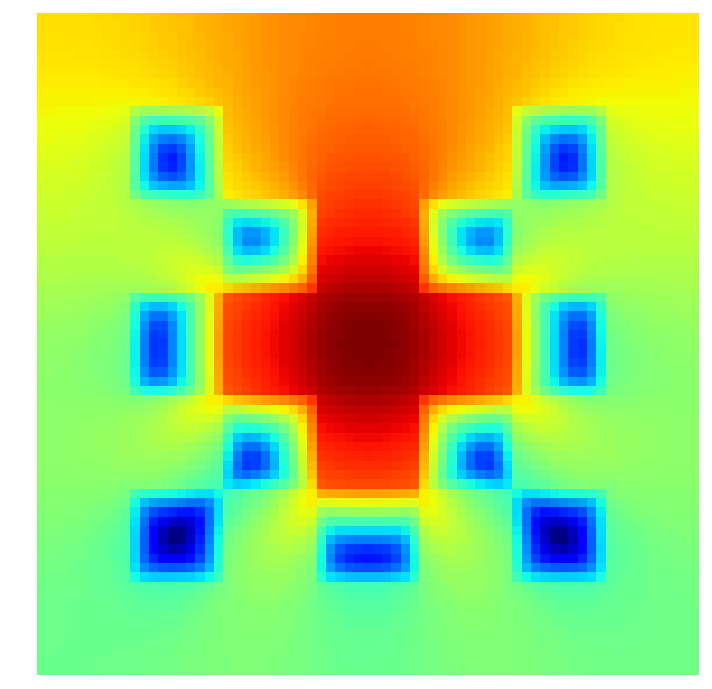
\includegraphics[width=\columnwidth]{04_pn_method/results/checkerboard2d_p5_neumann_staggered.png}
\caption{$P_1$-solution of the checkerboard problem.}
\label{fig:pn_staggering_correct_bc_checkerboard}
\end{subfigure}
\caption{Placing staggered grid coefficients such that the defined boundary interface is symmetric (left) leads to a correct symmetric solution of the checkerboard problem (right).}
\label{fig:pn_staggered_grid_handled_bc}
\end{figure}

The handling of boundary conditions is done by the solver framework. In order to support staggered grids, the stencil code will be generated with an additional function, which specifies the grid location of each coefficient. This function is used by the \emph{VoxelManager} to work out which additional unknowns are required. This results in complex management of indices of unknowns, as a simple indexing function is not sufficient anymore. Transparently handling this complexity is the purpose of the \emph{VoxelManager} class.

For client code applications, it is desirable to have all coefficients defined at the centers of voxels covering the problem domain. Therefore the solver framework offers an \emph{unstagger} function for staggered grids, which interpolates all coefficients at the voxel centers of the problem domain from the surrounding coefficient locations. Further the additional unknowns, which have been introduced to get correct boundary conditions, will be removed. This function converts a staggered grid solution vector to a collocated grid solution vector.

As shown in figure~\ref{fig:pn_staggering_correct_bc_checkerboard}, using the collocated grid from converting a staggered grid solution of a staggered grid solve, will produce a result free of oscillation and asymmetry artefacts.

\subsection{System Matrix and Solution}
\label{sec:pn_system_matrix}

After initializing the \emph{PNSystemBuilder} object matrix with the \emph{Stencil} and \emph{Scene}, the system matrix $A$ and right hand side vector $\vec{b}$ are built and made available to the client code, which will use it to solve for the solution vector $\vec{u}$. The solver developed as part of this thesis uses Eigen~\cite{Eigen}, but any other linear algebra package with standard methods available is applicable too. 

However, the system matrix $A$, when generated from the $P_N$-equations, has properties that restrict the application of methods for solving the system. The number of rows and columns of $A$ is determined by the total number of voxels in the computational domain, multiplied by the number of spherical harmonics coefficients per voxel. The matrix is squared and sparse due to the local structure of the discretization and coupling. Unfortunately, the system matrix $A$ is non-symmetric (due to the transport term) and not diagonal dominant, which together rules out many iterative methods for solving linear systems.
\begin{figure}[h]
\centering
%\missingfigure{structure of the system matrix and solution vector (the figure from the paper)}
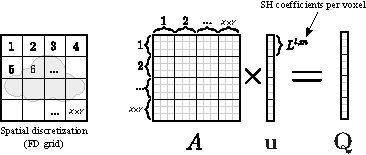
\includegraphics[width=0.75\textwidth]{04_pn_method/figures/fig_matrix_layout.pdf}
\caption{Structure of coefficient matrix $A$ and solution vector $\vec{u}$ after discretization of the $P_N$-equations on a finite difference grid.}
\label{fig:pn_matrix_layout}
\end{figure}

Some standard methods, such as LU-decomposition, QR-decomposition or Singular-value decomposition allow for solving systems of linear equations with non-symmetric coefficient matrices $A$ and are applicable to solving the system generated by the $P_N$-solver. 

Due to the asymmetry in $A$, applying iterative methods becomes a challenge. While iterative methods exist for non-symmetric matrices (based on Arnoldi iterations), these methods are more complex and tend to require more memory, that furthermore linearly grows with each operation. So only a limited number of iterations can be done before a restart becomes necessary.

Instead, iterative methods can be applied more easily by solving the normal form
\begin{align}
A^TA\vec{u} = A^T\vec{b}\ .
\end{align}
This gives a symmetric and positive definite system matrix $A^TA$, albeit with a higher condition number. Investigation of other solution schemes (e.g. multigrid) would be an interesting avenue for future work.

However, more importantly, in the presence of vacuum regions, matrix $A$ becomes singular and the system cannot be solved at all. The intuition behind this behavior is that in case of vacuum, the collision and scattering terms vanish completely, leaving the transport operator to exclusively define the solution. Since the transport operator only defines the relationship between unknowns in terms of their derivatives, it becomes clear that this is not enough information to constitute a unique solution. This is best exemplified by looking at a minimal version of that problem:
\begin{align*}
\frac{df\left(x\right)}{dx} = b\left(x\right)
\end{align*}
This differential equation imposes a constraint on the derivative of the solution, which is unique up to a constant factor. Hence there are infinitely many solutions. Therefore, there is no unique solution to this problem and hence the matrix $A$ after discretization will be singular.

A way out of this problem is to specify additional boundary conditions. However, for problems of simple complexity, this would already amount to finding a solution to the problem in the first place.

A simple alternative to which this thesis refers back is minimum thresholding. A minimum threshold value $\sigma_{min}$ is specified by the user. That threshold value is returned for any extinction value that falls below that threshold. This amounts to adding an ambient extinction medium by which vacuum regions are avoided completely and which causes the system to never become singular. Let $\sigma_{ot}$ be the original extinction coefficient coming from the input dataset. Unless stated otherwise, throughout this thesis the extinction coefficient is defined to be
\begin{align}
\label{eq:pn_solver_minimum_threshold}
\sigma_t\left(\vec{x}\right) =
\begin{cases}
\sigma_{ot}\left(\vec{x}\right), & \text{for $\sigma_{ot}\ge\sigma_{min}$}
\\
\sigma_{min}, & \text{otherwise}
\end{cases}
\end{align}

This concludes the section on the $P_N$-solver and its system components.


\section{Rendering Integration and Results}
\label{sec:pn_results}
